\documentclass[11pt,english,fleqn]{report}
\IfFileExists{t1futs.fd}{\usepackage{fourier}}{}
\IfFileExists{putb8a.pfb}{\usepackage{helvet}}{\usepackage{lmodern}}
\usepackage[T1]{fontenc}
\usepackage[latin9]{inputenc}
\setcounter{secnumdepth}{3}
\setcounter{tocdepth}{3}
\usepackage{babel}
\usepackage{verbatim}
\usepackage{graphicx}
\usepackage{url}
\usepackage{amsmath}
\usepackage{amssymb}

% MC STYLE
\usepackage[a4paper]{geometry}
\geometry{verbose,tmargin=3cm,bmargin=3cm,lmargin=3.5cm,rmargin=3.0cm}
\usepackage[pagestyles]{titlesec}
\usepackage[unicode,colorlinks,breaklinks]{hyperref}
\usepackage{float}
\usepackage{caption}
\usepackage[sort&compress,numbers]{natbib}
\usepackage{microtype}
\usepackage{etoolbox}
\setlength{\emergencystretch}{2em}

%%%%%%%%%%%%%%%%%%%%%%%%%%%%
% page layout
%%%%%%%%%%%%%%%%%%%%%%%%%%%%
\widowpenalty=200
\clubpenalty=200
\setlength{\parskip}{0.0ex plus 0.5ex minus 0.0ex}
% headings
\renewpagestyle{headings}[\small]{
\headrule \sethead{ %
{\ifnumgreater{\value{chapter}}{0}{Chapter \thechapter}{\bf \chaptertitle}} %
}{ %
{   \ifnumgreater{\value{chapter}}{0}{\bf \chaptertitle}{}} %
} %
{ \usepage}
}
\pagestyle{headings}

%empty page to pad chapters
\makeatletter
\def\cleardoublepage{\clearpage\if@twoside \ifodd\c@page\else
\hbox{}
\vspace*{\fill}
\begin{center}
\ 
\end{center}
\vspace{\fill}
\thispagestyle{empty}
\newpage
\if@twocolumn\hbox{}\newpage\fi\fi\fi}
\makeatother
%%%%%%%%%%%%%%%%%%%%%%%%%%%%
% spacings (use a lot of rubber lenghts)
%%%%%%%%%%%%%%%%%%%%%%%%%%%%
\setlength{\floatsep}{2ex plus 5ex minus 1ex }
\setlength{\textfloatsep}{3ex plus 3ex minus 1ex }

%%%%%%%%%%%%%%%%%%%%%%%%%%%%
% floats setup
%%%%%%%%%%%%%%%%%%%%%%%%%%%%
% positioning
\renewcommand{\topfraction}{0.85}
\renewcommand{\bottomfraction}{0.85}
\renewcommand{\textfraction}{0.15}
\renewcommand{\floatpagefraction}{0.65}
\setcounter{topnumber}{2}
\setcounter{bottomnumber}{2}
%default placement
\floatplacement{figure}{btp}
% caption
\captionsetup{margin=10pt,font=small,labelfont=bf}

%%%%%%%%%%%%%%%%%%%%%%%%%%%
% chapter headings
%%%%%%%%%%%%%%%%%%%%%%%%%%%
\titleformat{\chapter}[display]{\normalfont\huge\bfseries}%
{\vspace{1.5em}\raggedleft\large\chaptertitlename ~\thechapter\hrule\vspace{-0.5ex}}
{-0.25ex}{\begin{minipage}{0.75\textwidth}\raggedright}[\end{minipage}]
\makeatletter


%%%%%%%%%%%%%%%%%%%%%%%%%%%
% properties and fields formatting
%%%%%%%%%%%%%%%%%%%%%%%%%%%
% old version using ifthenelse
%\newcommand{\ipiitem}[3]{%   
%  \ifthenelse{ \equal{#1}{} } %
%             {} %
%             { \ifthenelse{ \equal{#1}{\underline{\smash{}}} } %
%                          {} %
%                          {  %
%      {\noindent\textbf{#1}:\rule{0.0pt}{1.05\baselineskip}\quad} % uses a strut to add a bit of vertical space
%                          } %
%             } %
%   {#2}\parskip=0pt\par
%   \ifthenelse{ \equal{#3}{} } %
%              {} %
%              { {\hfill\raggedleft\textit{\small #3}\par} }
%}

\newcommand{\ipiitem}[3]{%
   \ifblank{#1} % if no name is specified just output nothing
           {} %  
           { \ifstrequal{#1}{\underline{\smash{}}} % also in this case
             {} %
             { % print out beautifully
               {\noindent\textbf{#1}:\rule{0.0pt}{1.05\baselineskip}\quad} % uses a strut to add a bit of vertical space
             } %
           } %
    {#2}\parskip=0pt\par % prints the help text
   \ifblank{#3}{} %
          { {\hfill\raggedleft\textit{\small #3}\par} } % details string
}

\makeatletter
\newenvironment{ipifield}[4]{ %
   \ifblank{#1} {} {\vspace{0.5em}}  % some spacing between fields
   \noindent\parskip=0pt\begin{tabular}[t]{|p{1.0\linewidth}}   % table filling the whole line -- fields cannot break
      %cell without border
      \multicolumn{1}{@{}p{1.0\linewidth}}{
         \ipiitem{\underline{\smash{#1}}}{#2}{}  % name and help string
         \ifblank{#4} % if there are no attributes, write here the details
                 {  \ifblank{#3} {} % if there are any....
                            {{\hfill\raggedleft\textit{\small #3}}\par}}
                 {} %else do nothing here
         } \vspace{-1em}\\ % close multicol, go down and back up
      % cell with border (only if attributes are present)
      \ifblank{#4} {} % do nothing if there are no attributes (the details may just have been printed above
              { \ifblank{#3} {} { \vspace{-1em}{\hfill\raggedleft\textit{\small #3}}\par } % print the details
                {#4} \vspace{-1em} \\\hline } % negative vspace to undo the line break
   \end{tabular}
   \parskip=0pt\list{}{\listparindent 1.5em % indent the body of the environment 
         \leftmargin    \listparindent
         \rightmargin   0pt
         \parsep        0pt
         \itemsep       0pt
         \topsep        0pt
          }%
    \item\relax
 }
 {\endlist}
\makeatother

%%%%%%%%%%%%%%%%%%%%%%%%%%%%%% User specified LaTeX commands.
\usepackage{color}
\usepackage{multicol}\makeindex
\usepackage{xspace}
\usepackage[numbers]{natbib}

\newenvironment{code}{%
\footnotesize 
\verbatim
}{
\endverbatim
\normalsize
}

\makeatother

\begin{document}
\newcommand{\dd}{\; \mathrm{d}} 
\newcommand{\Tr}{\mathrm{Tr}} 
\newcommand{\bra}{< \! \!} 
\newcommand{\ket}{\! \! >} 
\newcommand{\betan}{\beta_N} 
\newcommand{\logn}{\mathrm{ln}} 
\newcommand{\expon}{\mathrm{exp}} 
\newcommand{\Imag}{\mathrm{Im}}
\newcommand{\ipi}{{i-PI}\xspace}
\newcommand{\DFT}{Quantum Espresso, CP2K, CPMD and FHI-AIMS }
\newcommand{\empirical}{LAMMPS}

\begin{titlepage} 

\begin{center}
\vspace*{2.5cm}

\par\end{center}

\begin{center}

\includegraphics[width=0.6\textwidth]{figures/ipi-logo.pdf}
\par\end{center}

\begin{center}
{\Large\bf A Python interface for \\Path Integral Molecular Dynamics}
\par\end{center}

\begin{center}
{\large v. 1.0}
\par\end{center}

\end{titlepage}

\pagenumbering{roman}

\tableofcontents{}


\newpage{}\pagenumbering{arabic}


\chapter{About \ipi}

\label{intro}

\ipi is a Path Integral Molecular Dynamics (PIMD) interface written
in Python, designed to be used together with an \emph{ab initio} evaluation
of the interactions between the atoms. The main goal is to decouple
the problem of evolving the ionic positions to sample the appropriate
thermodynamic ensemble and the problem of computing the inter-atomic
forces. 

\begin{figure}[hb]
\centering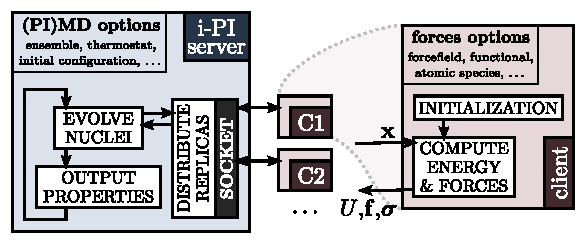
\includegraphics[width=0.9\textwidth]{figures/ipi-scheme.pdf}
\caption{\label{fig:scheme} Schematic representation of the functioning of \ipi{}.} 
\end{figure}

The implementation is based on a client-server paradigm, where \ipi
acts as the server and deals with the propagation of the nuclear dynamics,
whereas the calculation of the potential energy, forces and the potential
energy part of the pressure virial is delegated to one or more instances
of an external code, acting as clients. Since the main focus is on
performing \emph{ab initio} PIMD -- where the cost of the force evaluation
is overwhelming relative to the ionic dynamics -- clarity has been
privileged over speed. Still, the implementation of \ipi is efficient
enough that it can be used with empirical forcefields to perform simple
benchmarks and preparatory simulations. 


\section{Manual structure}

This manual will be structured as follows: 
\begin{itemize}
\item In chapter \ref{intro} we briefly discuss the basis for PIMD and
some of the specialized techniques used in \ipi. 
\item In chapter \ref{getstarted} we will discuss how to install 
and run the code, and test that it is working.
\item In chapter \ref{userguide} we explain in more detail the form of the input
and output files and how the communication between the client and
server codes is done.
\item In chapter \ref{hierarchy} a full list of the major classes used
in the code is given, along with the appropriate tag names and a brief
description of all the fields that can be specified in the xml input
file.
\item In chapter \ref{tutorial} we give a simple step-by-step walkthrough of
an example \ipi simulation.
\item In chapter \ref{trouble} we list some of the more commonly encountered
problems, and their solutions.
\end{itemize}

\section{Path Integral Molecular Dynamics}

Molecular dynamics (MD) is a technique used to study the properties
of a system of interacting particles by applying Newton's equations
of motion to produce trajectories which can be used to efficiently
explore the phase space. This can be used to calculate many equilibrium
and dynamical properties and to study systems from isolated gas molecules
to condensed phase bulk materials.

However, while this technique has been very successful, in most MD
implementations the assumption is made that the nuclei behave as classical
particles, which for light nuclei such as hydrogen is often a very
poor approximation as the effect of zero-point energy (ZPE) and quantum
tunnelling can be large. For example, even at room temperature the
vibrational frequency of an OH stretch in water is over 15 times larger
than the available thermal energy, and so this motion will be highly
quantized. The current state-of-the-art method to include nuclear
quantum effects (NQE) in the calculation of static properties of condensed
phase systems is path integral molecular dynamics (PIMD).

PIMD generates the quantum-mechanical ensemble of a system of interacting
particles by using MD in an extended phase space. This is derived
from the path integral formalism \cite{feyn-hibb65book}, which
relates the statistics of a collection of quantum particles to those
of a set of classical ring polymers, a ring polymer being a number
of replicas of a particle coupled by harmonic springs. This so-called
classical isomorphism is exact in the limit as the number of replicas
goes to infinity, but in practice is converged numerically with only
a finite number.

This then allows quantum phase space averages to be calculated from
classical trajectories, with only about an order of magnitude more
computing time than would be required for standard MD. Also, since
PIMD is simply classical MD in an extended phase space, many of the
techniques developed to improve the scope and efficiency of MD simulations
can be applied straightforwardly to the equivalent PIMD calculations
\cite{ceri+10jcp,mart+99jcp}. Finally, several techniques designed
specifically for PIMD simulations are now available to increase the
rate of convergence with respect to the number of replicas used 
\cite{mark-mano08jcp,ceri+11jcp,suzu95pla,chin97pla,ceri+12prsa,pere-tuck11jcp},
further reducing the computational overhead of the method. All
of these facts mean that it is now feasible to do PIMD simulations
with thousands of molecules, or even to use \emph{ab initio} electronic
structure calculations to propagate the dynamics for small systems.

Furthermore, the framework used to run PIMD simulations can be adapted
to generate approximate quantum dynamical information 
\cite{cao-voth93jcp,cao-voth94jcp,crai-mano04jcp,braa-mano06jcp},
and so can also be used to calculate correlation functions. While
real-time quantum coherences cannot be captured, the inclusion 
of quantum statistical information
and the rapid decoherence observed in condensed phase systems mean
that in many cases very accurate results can be obtained from such
approximate treatments of quantum dynamics \cite{habe+13arpc}.


\section{Implementation}


\subsection{Automated evaluation (depend objects)}

\ipi uses a caching mechanism with automatic value updating to make
the code used to propagate the dynamics as simple and clear as possible.
Every physical quantity that is referenced in the code is created
using a {}``depend'' object class, which is given the parameters
on which it depends and a function used to calculate its value. 

\begin{figure}[hpbt]
\centering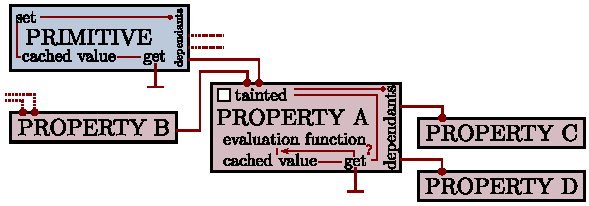
\includegraphics[width=0.9\textwidth]{figures/ipi-depend.pdf}
\caption{\label{fig:depend} Schematic overview of the functioning of the 
\emph{depend} class used as the base for properties and physical quantities in \ipi{}. 
A few ``primitive'' quantities -- such as atomic positions or momenta -- can be modified
directly. For most properties, one defines a function that can compute based on the
value of other properties. Whenever one property is modified, all the quantities that
depend on it are marked as tainted, so that -- when the value of one of the properties
is used, the function can be invoked and the updated value obtained. If a quantity
is not marked as tainted, the cached value is returned instead. 
}
\end{figure}


{}``Depend'' objects can be called to get the physical quantity
they represent. However, they have further functionality. Firstly,
once the value of a {}``depend'' object has been calculated, its
value is cached, so further references to that quantity will not need
to evaluate the function that calculates it. Furthermore, the code
keeps track of when any of the dependencies of the variable are updated,
and makes sure that the quantity is automatically recomputed when
it is needed. 

This choice makes implementation slightly more complex when the physical
observables are first introduced as variables, as one has to take
care of stating their dependencies as well as the function that computes
them. However, the advantage is that when the physical quantities
are used, in the integrator of the dynamics or in the evaluation of
physical properties, one does not need to take care of book-keeping
and the code can be clean, transparent and readable.


\begin{figure}[hpbt]
\centering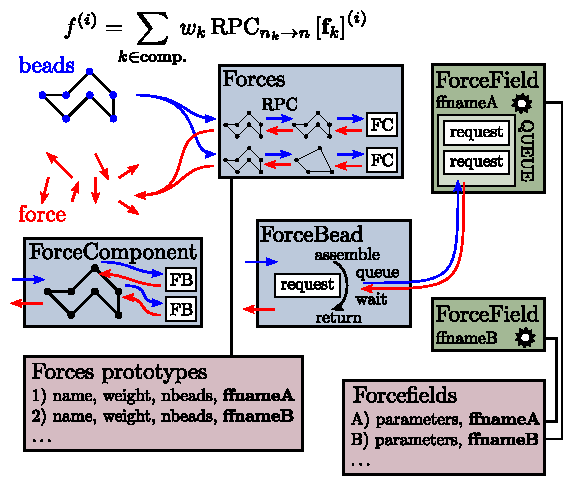
\includegraphics[width=0.9\textwidth]{figures/ipi-forces.pdf}
\caption{\label{fig:forces} Schematic representation of the different objects
that are involved in the evaluation of the forces. The multiple layers and complex
structure are necessary to give the possibility of decomposing the evaluation 
of the forces between multiple different clients and using different imaginary
time partitioning (e.g. one can compute the bonded interactions using one client,
and use a different client to compute the long-range electrostatic interactions,
contracted on a single bead~\cite{mark-mano08jcp}). 
}
\end{figure}


\subsection{Force evaluation}

Within \ipi{}, the evaluation of the forces plays a crucial role, 
as it is the step requiring communication with the client code. 
In order to have a flexible infrastructure that makes it possible
to perform simulations with advanced techniques such as ring-polymer
contraction~\cite{mark-mano08jcp}, the force evaluation machinery
in \ipi{} might appear complicated at first, and deserves a brief
discussion.

A scheme of the objects involved in the calculation of the forces
is presented in Figure~\ref{fig:forces}. The infrastracture comprises
a force provider class that deals with the actual subdivision of 
work among the clients, and a sequence of objects that translate
the request of the overall force of the system into atomic 
evaluations of one component of the force for an individual bead:
\ipi{} is built to hide the path integral infrastructure from the client, and so 
beads must be transferred individually.

Let us discuss for clarity a practical example -- a calculation 
of an empirical water model where the bonded interactions are 
computed on 32 beads by the program A, and the non-bonded interactions
are computed by client B, ring-polymer contracted on 8 beads.
Each client ``type'' is associated with a \hyperref[FORCEFIELD]{ForceField} 
object in the input. In the case of a \hyperref[FFSOCKET]{socket} interface,
the forcefield object specifies the address to which a client should connect,
and so multiple clients of type A or B can connect to \ipi{} at the same time.
Each forcefield object deals with queueing force evaluation requests
and computing them in a first-in-first-out fashion, possibly executing 
multiple requests in parallel. 

On the force evaluation side, the task of splitting the request of a
force evaluation into individual components and individual beads is 
accomplished by a chain of three objects, Forces, ForceComponent and ForceBead.
is the main force Forces evaluator, that is built from the prototypes
listed within the \hyperref[FORCES]{forces} field of \hyperref[SYSTEM]{system}.
Each \hyperref[FORCECOMPONENT]{force} item within the 
\hyperref[FORCES]{forces} tag describe one component of the force --
in our example one ForceComponent bound to a forcefield of type A, 
evaluated on 32 beads, and one ForceComponent bound to type B, evaluated
on 8 beads. Forces contains the machinery that automatically contracts the
actual ring polymer to the number of beads required by each component,
and combines the various components with the given weights to provide the 
overall force, energy and virial where required. 
ForceComponent is a very simple helper class that associates with each bead 
a ForceBead object, that is the entity in charge of filing force requests to
the appropriate ForceField object and waiting for completion of the
evaluation. 

\subsection{Communication protocol}

Since \ipi is designed to be used with a wide range of codes and
platforms, it has to rely on a simple and robust method for communicating
between the server and client. Even though other choices are possible,
and it should be relatively simple to implement other means of communication,
the preferred approach relies on sockets as the underlying infrastructure.
Both Internet and Unix domain sockets can be used: the latter allow
for fast communication on a single node, whereas the former make
it possible to realise a distributed computing paradigm, with clients
running on different nodes or even on different HPC facilities. In
order to facilitate implementation of the socket communication in
client codes, a simple set of C wrappers to the standard libraries
socket implementation is provided as part of the \ipi distribution,
that can be used in any programming language that can be linked with
C code.

As far as the communication protocol is concerned, the guiding principle
has been keeping it to the lowest common denominator, and avoiding
any feature that may be code-specific. Only a minimal amount of information
is transferred between the client and the server; the position of
the atoms and cell parameters in one direction, and the forces, virial
and potential in the other.

For more details about sockets and communication, see \ref{distrib}. 


\subsection{Internal units}

\label{units}

All the units used internally by \ipi are atomic units, as given
below. By default, both input and output data are given in atomic
units, but in most cases the default units can be overridden if one
wishes so. For details on how to do this, see \ref{inputunits} and
\ref{propertyfile}.

\texttt{
\begin{center}
\begin{tabular}{lll}
\hline\hline
Unit & Name & S.I. Value\\
\hline 
Length & Bohr radius & 5.2917721e-11 m\\
Time & N.A. & 2.4188843e-17 s\\
Mass & Electron mass & 9.1093819e-31 kg\\
Temperature & Hartree & 315774.66 K\\
Energy & Hartree & 4.3597438e-18 J\\
Pressure & N.A. & 2.9421912e13 Pa\\
\hline\hline
\end{tabular}
%\par\end{center}
\end{center}
}


\section{Core features}

The functionality of \ipi includes:
\begin{itemize}
\item Thermostats for constant temperature ensembles, including: \begin{itemize}
\item Local and global stochastic thermostats \cite{plangevin1908cras,buss-parr08cpc}, with optional optimized sampling of the ring polymer normal mode coordinates \cite{ceri+10jcp}.
\item Optimal sampling generalized Langevin equation (GLE) thermostats \cite{ceri+09jctc}.
\item Path integral + GLE (PI+GLE) thermostats \cite{ceri+11jcp} for accelerating the
convergence of the potential energy with respect to the number of replicas, 
as well as the more recent PIGLET method \cite{ceri-mano12prl}, which also
accelerates the convergence of the kinetic energy.
\end{itemize}
\item Barostats for constant pressure ensembles \cite{mart+99jcp,buss+09jpc}.
\item Ring polymer contraction \cite{mark-mano08jcp}.
\item Scaled path finite difference energy and heat capacity estimators
\cite{tyamamoto05jcp}.
\item Displaced path momentum distribution estimator \cite{linlin+10prl}.
\item Dynamical property calculation modes:\begin{itemize}
\item Ring polymer molecular dynamics \cite{crai-mano04jcp}.
\item Partially-adiabatic centroid molecular dynamics \cite{habe+08jcp,hone+06jcp}.
\end{itemize}
\end{itemize}

\section{Licence and credits}

Most of this code is distributed under the GPL licence. For more details see
\url{www.gnu.org/licences/gpl.html}. 
So that they can easily be incorporated in other codes, the files
in the directory {}``drivers'' are all held under the MIT licence.
For more details see \url{https://fedoraproject.org/wiki/Licensing:MIT}.

If you use this code in any
future publications, please cite this using {[}cpc paper citation{]}.

\subsection{Contributors}

\ipi was originally written by M. Ceriotti and J. More at Oxford University,
together with D. Manolopoulos. T. Spura and M. Rossi contributed to the 
initial development of the code, R. Distasio and B. Santra for helped creating patches for
Quantum Espresso.



\section{On-line resources}


\subsection{Python resources}

For help with Python programming, see \url{www.python.org}. For information
about the NumPy mathematical library, see \url{www.numpy.org}, and
for worked examples of its capabilities see \url{www.scipy.org/Tentative_NumPy_Tutorial}.
Finally, see \url{http://hgomersall.github.io/pyFFTW/} for documentation
on the Python FFTW library that is currently implemented with \ipi.


\subsection{Client code resources}

\label{librarywebsites}

There are currently client patches available for Quantum Espresso
and CP2K for all currently maintained versions. It should also 
be possible to adapt these patches
to other versions of the codes with minor modifications. For more
information about Quantum Espresso and CP2K, go to \url{www.quantum-espresso.org}
and \url{www.cp2k.org} respectively.

There is also a patch for the latest version of the LAMMPS empirical potential MD code.
More information on this code can be found at \url{http://lammps.sandia.gov/index.html}.

There are several Fortran and C libraries that most client codes will
probably need to run, such as FFTW, BLAS and LAPACK. These can be
found at \url{www.fftw.org}, \url{www.netlib.org/blas} and \url{www.netlib.org/lapack}
respectively.

These codes do not come as part of the \ipi package, and must be
downloaded separately. See chapter~\ref{clientinstall} for more details
of how to do this. 


\subsection{\ipi resources}

For more information about \ipi{} and to download the source code
go to \url{http://imx-cosmo.github.io/gle4md/ }, where one can also obtain colored-noise
parameters to run Path Integral with Generalized Langevin Equation
thermostat (PI+GLE/PIGLET) calculations.


\chapter{Getting started}

\label{getstarted}


\section{Installing \ipi}

\label{install}


\subsection{Requirements}

\ipi is Python code, and as such strictly speaking does not 
need to be compiled and installed. The {\tt i-pi} file in the
root directory of the distribution is the main (executable) script, 
and can be run as long as the system has installed:
\begin{itemize}
\item Python version 2.4 or greater
\item The Python numerical library NumPy
\end{itemize}
See \ref{runningsimulations} for more details on how to launch
\ipi.

Additionally, most client codes will have their own requirements.
Many of them, including the test client codes given in the {}``drivers''
directory, will need a suitable Fortran compiler. A C compiler is
required for the sockets.c wrapper to the sockets standard library.
Most electronic structure codes will also need to be linked with some
mathematical libraries, such as BLAS, FFTW and LAPACK. Installation
instructions for these codes should be provided as part of the code
distribution and on the appropriate website, as given in \ref{librarywebsites}.
Patching for use with \ipi{} should not introduce further dependencies.

\subsubsection{Using the setup.py module}

While the {\tt i-pi} file can be used to run any \ipi simulation, it
is often more convenient to install the package to the system's 
Python modules path, so that it is accessible by all users and can
be run without specifying the path to the Python script.

For this purpose we have included a module in the root directory of the \ipi
distribution, {\tt setup.py}, which handles creating a package with the 
executable and all the modules which are necessary for it to run.
The first step is to build the distribution using:

\begin{code}
> python setup.py build
\end{code}
Note that this requires the distutils package that comes with the
python-dev package. 

This creates a "build" directory containing only the files that
are used to run an \ipi simulation, which can then be used to create the
executable. This can be done in two ways,
depending on whether or not the user has root access. If the user does
have root access, then the following command will add the relevant source
files to the standard Python library directory:

\begin{code}
> python setup.py install
\end{code}
This will install the package in the /usr/lib/py\_vers directory,
where py\_vers is the version of Python that is being used.
This requires administrator priviledges.

Otherwise, one can install \ipi in a local Python path. If such 
path does not exist yet, one must create directories for the package to
go into, using:

\begin{code}
> mkdir ~/bin
> mkdir ~/lib/py_vers
> mkdir ~/lib/py_vers/site-packages
\end{code}

Next, you must tell Python where to find this library, by appending
to the Linux environment variable PYTHONPATH, using:

\begin{code}
> export PYTHONPATH=$PYTHONPATH:~/lib/py_vers/site-packages/
\end{code} 

Finally, the code can be installed using:

\begin{code}
> python setup.py install --prefix=~
\end{code}

Either way, it will now be possible to run the code automatically, using

\begin{code}
> i-pi input_file.xml
\end{code}

\subsection{\ipi download}

A tar file can be downloaded from the website \url{http://imx-cosmo.github.io/gle4md/}.
To install this you need to input the following command:

\begin{code}
> tar xf [ipi_tar_file.tar]
\end{code}


You can also obtain a local clone of the git repository (listed on \url{http://imx-cosmo.github.io/gle4md/}) using:

\begin{code}
> git clone [repository name]
\end{code}

The \ipi executable will run immediately, without needing to be installed
or compiled, but we include a setup.py module in the main directory so it can
be installed to the Python tree if so desired.

\subsection{Installing NumPy}

NumPy is the standard Python mathematics library, and is used for
most of the array manipulation and linear algebra in \ipi. It should
be installed alongside most standard Python environments on HPC facilities.
Otherwise, it is generally relatively straightforward to install it. 

In any case you must first obtain the NumPy code, which can be downloaded
as a tar file from \url{http://www.numpy.org}. If the version of
NumPy being installed is given by {}``np\_vers'', this can be extracted
using:

\begin{code}
> tar xzf np_vers.tar.gz
\end{code}

Before installing this code it first needs to be configured correctly.
Note that this requires the distutils package that comes with the
python-dev package. Assuming that the required software is installed,
the NumPy package is built using:

\begin{code}
> python setup.py build
\end{code}

The next step is to install NumPy. By default the download is to the
directory /usr/local. If you have root access, and so can write to
/usr, then all that needs to be done to finish the install is:

\begin{code}
> python setup.py install
\end{code}

If you do not have root access, then the next step depends on which
version of Python is beind used. With versions 2.6 or later there
is a simple command to automatically download into the directory \$HOME/local:

\begin{code}
> python setup.py install --user
\end{code}

With Python 2.4/2.5 the process is a little more involved. First you
must explicitly install the package in the directory of choice, {}``np\_dir''
say, with the following command:

\begin{code}
> python setup.py install --prefix=np_dir
\end{code}

Next, you must tell Python where to find this library, by appending
to the Linux environment variable PYTHONPATH. If you are
using Python version {}``py\_vers'', then the NumPy libraries will
have been installed in the directory {}``np\_dir/lib/py\_vers/site-packages'',
or a close analogue of this. In the above case the following command
will allow the Python interpreter to find the NumPy libraries:

\begin{code}
> export PYTHONPATH=$PYTHONPATH:np_dir/lib/py_vers/site-packages
\end{code}
%$

Now Python scripts can import the NumPy libraries using:

\begin{code}
import numpy
\end{code}


\subsection{PyFFTW}

Some of the steps in the dynamics algorithm involve a change of variables
from the bead coordinates to the normal modes of the ring polymers.
Currently, this transformation is, at least by default, computed using
a fast-Fourier transform (FFT) library within the NumPy distribution.
This however is not the only distribution that could be used, and
indeed faster stand-alone versions exist. The gold-standard FFT library
is the FFTW library, which is a set of C libraries that have been
heavily optimized for a wide range of applications. There have been
a number of Python wrappers built around the FFTW library, one of which
is currently interfaced with \ipi. This code can be found at \url{https://github.com/hgomersall/pyFFTW},
and has documentation at \url{http://hgomersall.github.io/pyFFTW/}.

This code has the following dependencies:
\begin{itemize}
\item Python version 2.7 or greater
\item Numpy version 1.6 or greater
\item FFTW version 3.2 or greater
\end{itemize}
This can be installed in the same way as NumPy, except using the code
distribution above, or using various installation packages as per
the instructions on the above documentation. Note that no other options
need to be specified in the input file; \ipi will check to
see if this library is available, and if it is it will be used by
default. Otherwise the slower NumPy version will be used.


\section{Installing clients}

\label{clientinstall}

\subsection{Patching CP2K}


You can download the source code for CP2K at \url{www.cp2k.org/}.
This can either be downloaded as a tar file, which
can be extracted in the same way as the Python and NumPy
libraries above, or via a svn client. 

As an example of the latter, CP2K version 2.4 can be downloaded to
a directory {}``cp2k-2.4'' using the command:

\begin{code}
> svn checkout svn://svn.code.sf.net/p/cp2k/code/branches/cp2k-2_4-branch cp2k-2.4
\end{code}

Before CP2K can run with \ipi, the code
must be adapted to use the socket interface. 
For this purpose \ipi is distributed with patch files in the
directory {}``patches''. When applied to a clean 
distribution, these will adjust the source code to make it
compatible with \ipi. 

For example, if we take CP2K 
version 2.4.0, and assuming that you are
currently in the top level directory of the CP2K distribution,
the patch can be applied to the source code using:

\begin{code}
> patch -p1 < ipidir/i-pi/patches/cp2k-2.4.0_ipi.patch
\end{code}
where ipidir is the directory containing the \ipi source code.

After this, continue the compilation as per the instructions at 
\url{www.cp2k.org/} to complete the install.
There are currently patches available for CP2K versions 2.4, 2.3, 2.2 and 2.1.

\subsection{Patching Quantum-Espresso}

You can download the source code for Quantum Espresso at \url{www.quantum-espresso.org/}
as a tar file. The tar file can be extracted in the same way as the Python and NumPy
libraries above. As for CP2K above, we include patch files to
adapt the Quantum Espresso source code so that it will work with \ipi.
Taking version 5.0 as an example, and again assuming you are in
the top level directory of the Quantum Espresso distribution,
this patch can be applied to the source code using:

\begin{code}
> patch -p1 < ipidir/i-pi/patches/espresso-5.0_ipi.patch
\end{code}

After this, continue the compilation as per the instructions at 
\url{www.quantum-espresso.org/} to complete the install.
There are currently patches available for 
Quantum Espresso versions 5.0, 4.3, 4.2 and 4.1.3.

\subsection{Patching LAMMPS}

You can download the source code for LAMMPS at \url{http://lammps.sandia.gov/index.html}.
This can either be downloaded as a tar file, which
can be extracted in the same way as the Python and NumPy
libraries above, via a svn client, which can be run in the
same way as for CP2K, or from a git repository, which can be downloaded
in the same way as for \ipi. 

As for CP2K above, we include patch files to
adapt the LAMMPS source code so that it will work with \ipi.
Currently we only provide a patch file for a recent 
version of LAMMPS, which can be applied to the source code using:

\begin{code}
> patch -p1 < ipidir/i-pi/patches/lammps-26Aug13_ipi.patch
\end{code}

After this, continue the compilation as per the instructions at 
\url{http://lammps.sandia.gov/index.html} to complete the install.
Note that the optional libraries CLASS2, KSPACE, MANYBODY and 
MOLECULE will all need to be included to run the examples provided
in the {}``examples'' directory.

\subsection{Writing a patch}

If you have edited a client code, and wish to make a patch available
for the new version, then this can be done very simply.
If your edited code is in a directory {}``new'', and a clean
distribution is held in a directory {}``old'', then a patch
{}``changes.patch'' can be created using:

\begin{code}
> diff -rupN old/ new/ > changes.patch
\end{code}

\section{Running \ipi}

\ipi functions based on a client-server protocol, where the evolution of the nuclear dynamics
is performed by the \ipi server, whereas the energy and forces evaluation is delegated to 
one or more instances of an external program, that acts as a client. This design principle
has several advantages, in particular the possibility of performing PIMD based on the forces
produced by one's favourite electronic structure/empirical force field code. However, it 
also makes running a simulation slightly more complicated, since the two components
must be set up and started independently.

\subsection{Running the \ipi server}

\label{runningsimulations}

\ipi simulations are run using the i-pi Python script found in the
{}``i-pi'' directory. This script takes an xml-formatted file as
input, and automatically starts a simulation as specified by the data
held in it. If the input file is called {}``input\_file.xml'', then
\ipi is run using:

\begin{code}
> python i-pi input_file.xml
\end{code}

This reads in the input data, initializes all the internally used
objects, and then creates the server socket. The code will then wait
until at least one client code has connected to the server before
running any dynamics. Note that until this has happened the code is
essentially idle, the only action that it performs is to periodically
poll for incoming connections.


\subsection{Running the client code}

\label{runningclients}

\subsubsection{Built-in, example client}

\label{driver.x}

While \ipi is designed with \emph{ab initio} electronic structure calculations
in mind, it also includes a Fortran empirical potential client code to do 
simple calculations and to run the examples.

The source code for this is included in the directory {}``drivers'', and can
be compiled into an executable {}``driver.x'' using the UNIX utility make.

This code currently has four empirical potentials hardcoded into it, 
a Lennard-Jones potential, the Silvera-Goldman potential \cite{silv-gold78jcp},
a 1D harmonic oscillator potential, and the ideal gas (i.e. no potential
interaction).

How the code is run is based on what command line arguments are passed to it.
The command line syntax is:

\begin{code}
> driver.x [-u] -h hostname -p port -m [gas|lj|sg|harm] -o parameters [-v]
\end{code}

The flags do the following:

\begin{description}
\item[-u:] Optional parameter. If specified, the client will connect to
a unix domain socket. If not, it will connect to an internet socket.
\item[-h:] Is followed in the command line argument list by the hostname
of the server.
\item[-p:] Is followed in the command line argument list by the port number
of the server.
\item[-m:] Is followed in the command line argument list by a string
specifying the type of potential to be used. {}``gas'' gives no potential,
{}``lj'' gives a Lennard-Jones potential, {}``sg'' gives a Silvera-Goldman
potential and {}``harm'' gives a 1D harmonic oscillator potential.
\item[-o:] Is followed in the command line argument list by a string of
comma separated values needed to initialize the potential parameters.
{}``gas'' requires no parameters, {}``harm'' requires a spring constant,
{}``sg'' requires a cut-off radius and {}``lj'' requires the length and
energy scales and a cut-off radius to be specified. All of these must
be given in atomic units. 
\item[-v:] Optional parameter. If given, the client will print out
more information each time step.
\end{description}

This code should be fairly simple to extend to other pair-wise interaction
potentials, and examples of its use can be seen in the {}``examples'' 
directory, as explained in \ref{tests}.

\subsubsection{CP2K}

To use CP2K as the client code using an 
internet domain socket on the host
address {}``host\_address'' and on the port number {}``port''
the following lines must be added to its input file:

\begin{code}
&GLOBAL
   ...
   RUN_TYPE DRIVER
   ...
&END GLOBAL

&MOTION
   ...
   &DRIVER
      HOST host_address
      PORT port
   &END DRIVER
   ...
&END MOTION
\end{code}

If instead a unix domain socket is required then the following
modification is necessary:

\begin{code}
&MOTION
   ...
   &DRIVER
      HOST host_address
      PORT port
      UNIX
   &END DRIVER
   ...
&END MOTION
\end{code}

The rest of the input file should be the same as for a standard CP2K 
calculation, as explained at \url{www.cp2k.org/}.

\subsubsection{Quantum-Espresso}

To use Quantum-Espresso as the client code using an 
internet domain socket on the host
address {}``host\_address'' and on the port number {}``port''
the following lines must be added to its input file:

\begin{code}
&CONTROL
   ...
   calculation=`driver'
   srvaddress=`host_address:port'
   ...
/
\end{code}

If instead a unix domain socket is required then the following
modification is necessary:

\begin{code}
&CONTROL
   ...
   calculation=`driver'
   srvaddress=`UNIX:host_address:port'
   ...
/
\end{code}

The rest of the input file should be the same as for a standard Quantum
Espresso calculation, as explained at \url{www.quantum-espresso.org/}.

\subsubsection{LAMMPS}

To use LAMMPS as the client code using an 
internet domain socket on the host
address {}``host\_address'' and on the port number {}``port''
the following lines must be added to its input file:

\begin{code}
fix 1  all driver host_address port
\end{code}

If instead a unix domain socket is required then the following
modification is necessary:

\begin{code}
fix 1  all driver host_address port unix
\end{code}

The rest of the input file should be the same as for a standard LAMMPS 
calculation, as explained at \url{http://lammps.sandia.gov/index.html}.

\subsection{Running on a HPC system}\label{hpc}

Running \ipi on a high-performance computing (HPC) system can be a bit more challenging
than running it locally using UNIX-domain sockets or using the \emph{localhost} 
network interface.
The main problem is related to the fact that different HPC systems adopt
a variety of solutions to have the different nodes communicate with each other
and with the login nodes, and to queue and manage computational jobs. 
 
\begin{figure}[hbt]
\centering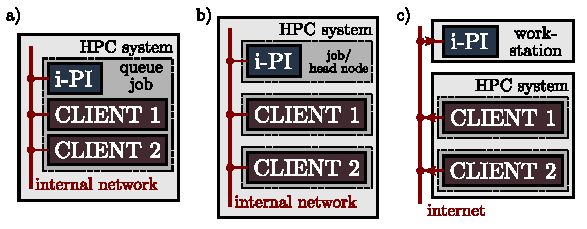
\includegraphics[width=0.9\textwidth]{figures/ipi-running.pdf}
\caption{\label{fig:running} Different approaches to run \ipi and a number of 
instances of the forces code on a HPC system: a) running \ipi and the clients in a single
job; b) running \ipi and the clients on the same system, but using different jobs, or running
\ipi interactively on the login node; c) running \ipi on a local workstation, communicating
with the clients (that can run on one or multiple HPC systems) over the internet. } 
\end{figure}

Figure~\ref{fig:running} represents schematically three different approaches
to run \ipi on a HPC system:
\begin{enumerate}
\item running both \ipi{} and multiple instances of the client as a single job on 
the HPC system. The job submission script must launch \ipi{} first, as a serial
background job, then wait a few seconds for it to load and create a socket
\begin{code}
> python i-pi input_file.xml &> log & wait 10
\end{code}
Then, one should launch with mpirun or any system-specific mechanism 
one or more independent instances of the client code. Note that not all
queing systems allow launching several mpirun instances from a single job.
\item running \ipi{} and the clients on the HPC system, but in separate jobs.
Since \ipi{} consumes very little resources, one should ideally launch it 
interactively on a login node 
\begin{code}
> nohup python i-pi input_file.xml < /dev/null &> log & 
\end{code}
or alternative on a queue with a very long wall-clock time. 
Then, multiple instances of the client can be run as independent jobs:
as they start, they will connect to the server which will take care of
adding them dynamically to the list of active clients,
dispatching force calculations to them, and removing them from the list
when their wall-clock time expires. This is perhaps the model
that applies more easily to different HPC systems; however it requires
having permission to run on the head node, or having access to a long
wall-clock time queue that ensures that \ipi is always active. 
\item running \ipi{} on a simple workstation, and performing 
communication over the internet with the clients that run on one
or more HPC systems. This model exploits in full the distributed-computing
model that underlies the philosophy of \ipi and is very robust --
as the server can be always on, and the output of the simulation is 
generated locally. However, this is also the most complicated to set up,
as the local workstation must accept in-coming connections 
from the internet -- which is not always possible when behind a 
 firewall -- and the compute nodes of the HPC centre must have
an outgoing connection to the internet, which often requires ssh tunnelling
through a login node (see section~\ref{distrib} for more details). 
\end{enumerate}
\section{Testing the install}

\label{tests}

\subsection{test the installation with `nose`}

There are several test cases included, that can be run automatically with
`nosetests` from the root directory.

\begin{code}
> nosetests -v
\end{code}

\subsection{test cases with input files}

Several test cases are distributed with the code to ensure that your
distribution is working correctly. There are also simple tests to
see if the client codes are working correctly.

All the input files are contained in the directory {}``examples'', which is
subdivided into the following directories:
\begin{description}
\item[{tutorial:}] Contains the input files needed to run the
tutorial in \ref{tutorial}.
\item [{lj:}] This gives a simple classical Lennard-Jones simulation of
Ne. The state points are given by (\(N\), \(\rho\), \(T\)) = (864, 0.35,
1.62), (\(N\), \(\rho\), \(T\)) = (864, 0.75, 1.069) and (\(N\), \(\rho\), \(T\))
= (864, 0.88, 1.095) in reduced Lennard-Jones units, so that the results
can be compared to those in \cite{lverlet67pr}.
\item [{ph2:}] This simulates para-hydrogen using the isotropic Silvera-Goldman
pair potential \cite{silv-gold78jcp}. There are three directories, {}``RPMD'', {}``nvt''
and {}``Tuckerman''. {}``RPMD'' and {}``nvt'' have tests which
can be compared to the results of \cite{mill-mano05jcp}, and {}``Tuckerman''
has tests which can be compared to the results of \cite{mart+99jcp}.
\item [{qespresso:}] This has two simple examples to test to see if the Quantum-Espresso
client is functioning correctly. There is one simple 4-atom lithium
test, and a test using a single water molecule.
\item [{harmonic:}] This has a simple example of a 1D harmonic oscillator.
This demonstrates the displaced path integral momentum distribution
estimator as given in \cite{linlin+10prl}. As the momentum distribution
is known analytically for this simple system, this provides an indication
of how well the method is working.
\item [{lammps:}] This has a simple implementation of the q-TIP4P-F empirical
water model of \cite{habe+09jcp} using the classical molecular dynamics
code LAMMPS. It demonstrates both the convergence of the PIGLET method
\cite{ceri-mano12prl}, as well as the use of ring-polymer contraction
methods \cite{mark-mano08jcp}.

This also contains one example using LAMMPS to calculate the interactions
between carbon atoms in graphene. This uses the optimized Tersoff 
parameters for carbon given in \cite{lind-broi10prb,errlind-broi10prb}.
\item [{cp2k:}] Contains the tests for the CP2K client code. Holds input files
to run the high-pressure water calculations 
presented in [cpc publication citation].
\end{description}

\chapter{User guide}

\label{userguide}


\section{Input files}


\subsection{Input file format and structure}

\label{ifilestructure}

In order to give the clearest layout, xml formatting was chosen as
the basis for the main input file. An xml file consists of
a set of hierarchically nested tags. There are three parts to an xml
tag. Each tag is identified by a tag name, which specifies the class
or variable that is being initialized. Between the opening and closing
tags there may be some data, which may or may not contain other tags.
This is used to specify the contents of a class object,
or the value of a variable. Finally tags can have attributes,
which are used for metadata, i.e. data used to specify
how the tag should be interpreted. As an example, a `mode' attribute can 
be used to select between different thermostatting algorithms,
specifying how the options of the thermostat class should be interpreted.

A xml tag has the following syntax:

\begin{code}
<tag_name attribute_name='attribute_data'>tag_data</tag_name>
\end{code}

The syntax for the different types of tag data is given below: 

\texttt{
\begin{center}
\begin{tabular}{cc}
\hline\hline
Data type & Syntax\\
\hline 
Boolean & <tag>True</tag> or <tag>False</tag>\\
Float & <tag>11.111</tag> or <tag>1.1111e+1</tag>\\
Integer & <tag>12345</tag>\\
String & <tag>string\_data</tag>\\
Tuple & <tag> (int1, int2, \ldots )</tag>\\
Array & <tag> {[} entry1, entry2, \ldots {]} </tag>\\
Dictionary & <tag>\{name1: data1, name2: data2, \ldots \}</tag>\\
\hline\hline
\end{tabular}
\end{center}
}

Note that arrays are always given as one-dimensional lists. In cases
where a multi-dimensional array must be entered, one can use the `shape'
attribute, that determines how the list will be reshaped into a multi-dimensional
array. For example, the bead positions are
represented in the code as an array of shape 
(number of beads, 3*number of atoms). If we take a system with 20 atoms
and 8 beads, then this can be represented in the xml input file as:

\begin{code}
<beads nbeads='8' natoms='20'>
   <q shape=`(8,60)'>[ q11x, q11y, q11z, q12x, q12y, ... ]</q>
   ...
</beads>
\end{code}

If `shape' is not specified, a 1D array will be assumed.

The code uses the hierarchical nature of the xml format to help read the data; if
a particular object is held within a parent object in the code, then
the tag for that object will be within the appropriate parent tags.
This is used to make the structure of the simulation clear. 

For example,
the system that is being studied is partly defined by the thermodynamic
ensemble that should be sampled, which in turn may be partly defined
by the pressure, and so on. To make this dependence clear in the code
the global simulation object which holds all the data contains
an ensemble object, which contains a pressure variable.
 
Therefore the input file is specified
by having a {}``\hyperref[SIMULATION]{simulation}'' tag, containing an 
{}``\hyperref[ENSEMBLE]{ensemble}''
tag, which itself contains a {}``pressure'' tag, which will contain
a float value corresponding to the external pressure. In this
manner, the class structure can be constructed iteratively.

For example, suppose we want to generate a \emph{NPT} ensemble at an external
pressure of \(10^{-7}\) atomic pressure units. This would be specified by
the following input file:

\begin{code}
<simulation>
   <ensemble mode='npt'>
      <pressure> 1e-7 </pressure>
      ...
   </ensemble>
   ...
</simulation>
\end{code}

To help detect any user error the recognized tag names, data types
and acceptable options are all specified in the code in a specialized
input class for each class of object. A full list of all the available
tags and a brief description of their function is given in chapter~\ref{hierarchy}.


\subsubsection{Overriding default units}

\label{inputunits}

Many of the input parameters, such as the pressure in the above example,
can be specified in more than one unit. Indeed, often the atomic unit
is inconvenient to use, and we would prefer something else. Let us
take the above example, but instead take an external pressure of 3
MPa. Instead of converting this to the atomic unit of pressure, it
is possible to use pascals directly using:

\begin{code}
<simulation>
   <ensemble mode=`npt'>
      <pressure units=`pascal'> 3e6 </pressure>
      ...
   </ensemble>
   ...
</simulation>
\end{code}

The code can also understand S.I. prefixes, so this can be simplified
further using:

\begin{code}
<simulation>
   <ensemble mode='npt'>
      <pressure units=`megapascal'> 3 </pressure>
      ...
   </ensemble>
   ...
</simulation>
\end{code}

A full list of which units are defined for which dimensions
can be found in the units.py module.


\subsection{Initialization section}

The input file can contain a {}``\hyperref[INITIALIZER]{initialize}'' tag, which
contains a number of fields that determine the starting values of the various
quantities that define the state of the simulation -- atomic positions, cell parameters, velocities, \ldots.
These fields (\hyperref[INITPOSITIONS]{positions},  \hyperref[INITVELOCITIES]{velocities},  
\hyperref[INITCELL]{cell},  \hyperref[INITMASSES]{masses},  \hyperref[INITLABELS]{labels},
\hyperref[INITFILE]{file}) specify how the values should be obtained: 
either from a manually-input list or from an external file.   

\subsubsection{Configuration files}

\label{configfile}

Instead of initializing the atom positions manually, the starting
configuration can be specified through a separate data file. The name
of the configuration file is specified within one of the possible
fields of an {}``\hyperref[INITIALIZER]{initialize}'' tag. 
The file format is specified with the  {}``mode'' attribute.
The currently accepted file formats are:
\begin{itemize}
\item pdb
\item xyz
\item chk
\end{itemize}
the last of which will be described in the next section.

Depending on the field name, the values read from the external file will 
be used to initialize one component of the simulation or another (e.g. the positions
or the velocities). The \hyperref[INITFILE]{file} tag can be used as a shortcut 
to initialize the atom positions, labels, masses and possibly
the cell parameters at the same time. For instance, 

\begin{code}
<initialize nbeads="8">
   <file mode="pdb"> init.pdb </file>
</initialize>
\end{code}

\noindent is equivalent to

\begin{code}
<initialize nbeads="8">
   <positions mode="pdb"> init.pdb </positions>
   <labels mode="pdb"> init.pdb </labels>
   <masses mode="pdb"> init.pdb </masses>
   <cell mode="pdb"> init.pdb </cell>
</initialize>
\end{code}

In practice, the using the \hyperref[INITFILE]{file} tag will only read the information that
can be inferred from the given file type, so for an `xyz' file, the cell
parameters will not be initialized. 


\subsubsection{Initialization from checkpoint files}

\ipi gives the option to output the entire state of the simulation at
a particular timestep as an xml input file, called a checkpoint file
(see \ref{checkpoint} for details). As well as being a valid input
for \ipi{},  a checkpoint can also be used inside an 
``\hyperref[INITIALIZER]{initialize}'' tag to specify the configuration
of the system, discarding other parameters of the simulation such as
the current time step or the chosen ensemble. 
Input from a checkpoint is selected 
by using {}``chk'' as the value of the {}``mode'' attribute. As
for the configuration file, a checkpoint file can be used to initialize
either one or many variables depending on which tag name is used.

\section{Output files}

\label{outputfiles}

\ipi uses a very flexible mechanism to specify how and how often
atomic configurations and physical properties should be output. Within
the {}``\hyperref[OUTPUTS]{output}'' tag of the xml input 
file the user can specify multiple tags, each one of 
which will correspond to a particular output
file. Each file is managed separately by the code, so what is output
to a particular file and how often can be adjusted for different files independently.

For example, some of the possible output properties require more than
one force evaluation per time step to calculate, and so can considerably
increase the computational cost of a simulation unless they are computed
once every several time steps. On the other hand,
for properties such as the conserved energy quantity it is easy, and
often useful, to output them every time step as they are simple to
compute and do not take long to output to file. 

There are three types of output file that can be specified; property
files for system level properties, trajectory files for atom/bead
level properties, and checkpoint files which save the state of the
system and so can be used to restart the simulation from a particular
point. For a brief overview of the format of each of these types of
files, and some of their more common uses, see \ref{part1}.
To give a more in depth explanation of each of these files, 
they will now be considered in turn.


\subsection{Properties}

\label{propertyfile}

This is the output file for all the system and simulation level properties,
such as the total energy and the time elapsed. It is designed to 
track a small number of important properties throughout a
simulation run, and as such has been formatted to be used as input
for plotting programs such as gnuplot.

The file starts with
a header, which describes the properties being written in the different
columns and their output units. This is followed by the actual
data. Each line corresponds to one instant of the simulation.
The file is fixed formatted, with two blank characters at the start
of each row, then the data in the same order as the header row. By default, each
column is 16 characters wide and every float is written in exponential
format with 8 digits after the decimal point.

For example, if we had asked for the current time step, the total
simulation time in picoseconds, and the potential energy in electronvolt,
then the properties output file would look something like:

\begin{code}
# column   1     --> step : The current simulation time step.
# column   2     --> time{picosecond} : The elapsed simulation time.
# column   3     --> potential{electronvolt} : The physical system potential energy.
    0.00000000e+00     0.00000000e+00    -1.32860475e+04
    1.00000000e+00     1.00000000e-03    -1.32865789e+04
...
\end{code}

The properties that are output are determined by the 
{}``\hyperref[PROPERTIES]{properties}''
tag in the xml input file. The format of this tag is:

\begin{code}
<properties stride=`' filename=`' flush=`' shape=`'>
   [ prop1name{units}(arg1; ... ), prop2name{...}(...), ...  ]
</properties>
\end{code}

\noindent e.g.

\begin{code}
<properties stride=`100' filename=`output'>
   [ step, atom_x{angstrom}(index=2;bead=0) ]
</properties>
\end{code}

The attributes have the following meanings:
\begin{description}
\item [{stride}] The number of steps between each output to file
\item [{filename}] The name of the output file
\item [{flush}] The number of output lines between buffer flushes
\item [{shape}] The number of properties in the list.
\end{description}
The tag data is an array of strings, each of which contains three
different parts:
\begin{itemize}
\item The property name, which describes which type of property is to be
output. This is a mandatory part of the string.
\item The units that the property will be output in. These are specified
between curly brackets. If this is not specified, then the property
will be output in atomic units. Note that some properties can only
be output in atomic units.
\item The arguments to be passed to the function. These are specified between
standard brackets, with each argument separated by a semi-colon. These
may or may not be mandatory depending on the property, as some arguments
have well defined default values. The arguments
can be specified by either of two different syntaxes, (name1=arg1;
\ldots ) or (arg1; \ldots ). 

The first syntax uses keyword arguments. The above example would set the variable
with the name {}``name1'' the value {}``arg1''. 
The second syntax uses positional arguments. This syntax
relies on the arguments being specified in the correct order, as defined
in the relevant function in the property.py module, since the user has
not specified which variable to assign the value to. 

The two syntaxes
may be mixed, but positional arguments must be specified first otherwise
undefined behaviour will result. If no arguments are specified, then
the defaults as defined in the properties.py module will be used.
\end{itemize}
The different available properties are:

\input{input_docs/property_list}

\subsection{Trajectory files} \label{trajectories}

These are the output files for atomic or bead level properties, such
as the bead positions. In contrast to properties files, they output data for 
all atomic degrees of freedom, in a format that can be read by visualization packages
such as VMD.

Multiple trajectory files can be specified, each described by a separate
{}``\hyperref[TRAJECTORY]{trajectory}'' tag within the 
``\hyperref[OUTPUTS]{output}'' section of the input file. 
The allowable file formats for the trajectory output files are the same as for the configuration
input files, given in~\ref{configfile}.

These tags have the format:

\begin{code}
<trajectory stride=`' filename=`' format=`' cell_units=`' flush=`' bead=`'>
   traj_name{units}(arg1;...)
</trajectory>
\end{code}

This is very similar to the 
{}``\hyperref[PROPERTIES]{properties}'' tag, except that it has the
additional tags {}``format'' and {}``cell\_units'', and only one
\emph{traj\_name} quantity can be specified per file. `format' specifies the format
of the output file, and `cell\_units' specifies the units in which
the cell dimensions are output. 
Depending on the quantity being output, the trajectory may consist of just 
one file per time step (e.g. the position of the centroid) or of several files, 
one for each bead, whose name will be automatically determined by 
appending the bead index to the specified  {}``filename'' attribute (e.g. 
the beads position). 
In the latter case it is also possible to output the quantity computed
for a single bead by specifying its (zero-based) index in the {}``bead'' attribute. 

The quantities that can be output in trajectory files are:

\input{input_docs/trajectory_list}


\subsection{Checkpoint files}

\label{checkpoint}

As well as the above output files, the state of the system at a particular
time step can also be saved to file. These checkpoint files can later be
used as input files, with all the information required to restore
the state of the system to the point at which the file was created. 

This is specified by the {}``\hyperref[CHECKPOINT]{checkpoint}'' tag
which has the syntax:

\begin{code}
<checkpoint stride=`' filename=`' overwrite=`'>
   step
</checkpoint>
\end{code}

Again, this is similar to the {}``\hyperref[TRAJECTORY]{trajectory}'' and 
{}``\hyperref[PROPERTIES]{properties}''
tags, but instead of having a value which specifies what to output,
the value simply gives a number to identify the current checkpoint
file. There is also one additional attribute, {}``overwrite'', which
specifies whether each new checkpoint file overwrites the old one,
or whether all checkpoint files are kept. If they are kept, they will
be written not to the file {}``filename'', but instead an index
based on the value of {}``step'' will be appended to it to distinguish
between different files.

If the `step' parameter is not specified, the following syntax can
also be used:

\begin{code}
<checkpoint stride=`' filename=`' overwrite=`'/>
\end{code}


\subsubsection{Soft exit and RESTART}

As well as outputting checkpoint files during a simulation run, \ipi{} also
creates a checkpoint automatically at the end of the simulation, with
file name {}``RESTART''. In the same way as the checkpoint files discussed 
above, it contains the full state of the simulation. 
It can be used to seamlessly restart the simulation if the user decides 
that a longer run is needed to gather sufficient statistics, or if \ipi{} is terminated
before the desired number of steps have been completed.

\ipi will try to generate a RESTART file when it terminates, either because
\emph{total\_time} has elapsed, or because it received a (soft) kill signal 
by the operating system. A soft exit can also be forced by creating 
an empty file named ``EXIT'' in
the directory in which \ipi is running. 

An important point to note is that since each time step is split into
several parts, it is only at the end of each step that all the
variables are consistent with each other in such a way that the simulation
can be restarted from them without changing the dynamics. Thus if
a soft exit call is made during a step, then the restart file that
is created must correspond to the state of the system \emph{before} 
that step began. To this end, the state of the system is saved at the
start of every step.


\section{Distributed execution}

\label{distrib}

\subsection{Communication protocol}

\ipi is based on a clear-cut separation between the 
evolution of the nuclear coordinates and the evaluation of energy
and forces, which is delegated to an external program.
The two parts are kept as independent as possible, to minimize
the client-side implementation burden, and to make sure that the 
server will be compatible with any empirical or \emph{ab initio} code that 
can compute inter-atomic forces for a given configuration.

Once a communication channel has been established between the 
client and the server (see \ref{sockets}), the two parties
exchange minimal information: \ipi{} sends the atomic positions
and the cell parameters to the client, which computes energy, forces
and virial and returns them to the server. 

The exchange of information is regulated by a simple 
communication protocol. The server polls the status of the client,
and when the client signals that is ready to compute forces 
\ipi sends the atomic positions to it. When the client responds to the
status query by signalling that the force evaluation is finished,
\ipi will prepare to receive the results of the calculation.
 If at any stage the client does not respond to a query, the server 
will wait and try again until a prescribed timeout period has elapsed, 
then consider the client to be stuck, disconnect from it 
and reassign its force evaluation task to another active instance. 
The server assumes that 4-byte integers, 8-byte floats
and 1-byte characters are used. The typical communication flow is
as follows:
%
\begin{enumerate}
\item a header string {}``\textbf{STATUS}'' is sent by the server to 
the client that has connected to it;
\item a header string is then returned, giving the status of the client
code. Recognized messages are:
\begin{description}
\item [{{}``NEEDINIT'':}] if the client code needs any initialising data,
it can be sent here. The server code will then send a header string
{}``INIT'', followed by an integer corresponding to the bead index,
another integer giving the number of bits in
the initialization string, and finally the initialization string itself.
\item [{{}``READY'':}] sent if the client code is ready to calculate
the forces. The server socket will then send a string {}``POSDATA'',
then nine floats for the cell vector matrix, then another nine floats
for the inverse matrix. The server socket will then send one
integer giving the number of atoms, then the position data as 3 floats
for each atom giving the 3 cartesian components of its position.
\item [{{}``HAVEDATA'':}] is sent if the client has finished computing the
potential and forces. The server socket then sends a string {}``GETFORCE'',
and the client socket returns {}``FORCEREADY''. The potential is
then returned as a float, the number of atoms as an integer, then
the force data as 3 floats per atom in the same way as the positions,
and the virial as 9 floats in the same way as the cell vector matrix. 
Finally, the client may return an arbitrary string containing additional
data that have been obtained by the electronic structure calculation 
(atomic charges, dipole moment, \ldots). The client first returns
an integer specifying the number of characters, and then the string,
which will be output verbatim if this ``extra'' information is
requested in the output section (see \ref{trajectories}).

\end{description}
\item The server socket waits until the force data for each replica of the
system has been calculated and returned, then the MD can be propagated for
one more time step, and new force requests will be dispatched.
\end{enumerate}

\subsection{Parallelization}

As mentioned before, one of the primary advantages of using this type
of data transfer is that it allows multiple clients to connect
to an \ipi server, so that different replicas of the system can be
assigned to different client codes and their forces computed in parallel.
In the case of \emph{ab initio} force evaluation, this is a trivial
level of parallelism, since the cost of the force calculation
is overwhelming relative to the overhead involved in exchanging 
coordinates and forces. Note that even if the parallelization over
the replicas is trivial, often one does not obtain perfect scaling,
due to the fact that some of the atomic configurations might require
more steps to reach self-consistency, and the wall-clock time per step
is determined by the slowest replica.

\ipi maintains a list of active clients, and distributes the forces
evaluations among those available. This means that, if desired, one 
can run an $n$-bead calculation using only $m<n$ clients, as the 
server takes care of sending multiple replicas to each client per 
MD step. To avoid having clients idling for a substantial amount
of time, $m$ should be a divisor of $n$. The main advantage of 
this approach, compared to one that rigidly assigns one instance of
the client to each bead, is that if each client is run as an independent
job in a queue (see~\ref{hpc}), \ipi can start performing PIMD
as soon as a single job has started, and can carry on advancing the
simulation even if one of the clients becomes unresponsive.

Especially for \emph{ab initio} calculations, there is an advantage
in running with $m=n$. \ipi will always try to send the coordinates for one
path integral replica to the client that computed it at the previous 
step: this reduces the change in the particle positions between 
force evaluations, so that the charge density/wavefunction from the 
previous step is a better starting guess and self-consistency can be 
achieved faster. Also, receiving coordinates that represent a continuous
trajectory makes it possible to use extrapolation
strategies that might be available in the client code.

Obviously, most electronic-structure client codes provide a further level
of parallelisation, based on OpenMP and/or MPI. This is fully compatible with
\ipi, as it does not matter how the client does the calculation since
only the forces, potential and virial are sent to the server, and the communication
is typically performed by the master process of the client. 


\subsection{Sockets} \label{sockets}

The communication between the \ipi server and the client code that
evaluates forces is implemented through sockets. A socket is a 
data transfer device that is designed for internet communication,
so it supports both multiple client connections to the same server and
two-way communication. This makes sockets ideal for use in \ipi,
where each calculation may require multiple instances of the client code. 
A socket interface can actually function in two different modes.

UNIX-domain sockets are a mechanism for local, inter-process
communication. They are fast, and best suited when one wants
to run \ipi  with empirical potentials, and the latency of the 
communication with the client becomes a significant overhead
for the calculation. UNIX-domain sockets create a special file
in the local file system, that serves as a rendezvous point
between server and clients, and are uniquely identified by the
name of the file itself, that can be specified in the ``address'' tag of 
``\hyperref[FFSOCKET]{socket}'' in the xml input file and in 
the input of the client.

Unfortunately, UNIX sockets do not allow one to run \ipi{} and 
the clients on different computers, which limits greatly their 
utility when  one needs to run massively parallel calculations. 
In these cases -- typically when performing \emph{ab initio} 
simulations -- the force calculation becomes the bottleneck, so there is no
need for fast communication with the server, and one can 
use internet sockets, that instead are specifically designed
for communication over a network.

Internet sockets are described by an address and a port number.
The address of the host is given as the IP address,
or as a hostname that is resolved to an IP address by a domain name server,
and is specified by the {}``address'' variable of a 
\hyperref[FFSOCKET]{socket} object. 
The port number is an integer between 1 and 65535 used to distinguish
between all the different sockets open on a particular host. As
many of the lower numbers are protected for use in important system
processes or internet communication, it is generally advisable to
only use numbers in the range 1025-65535 for simulations.

The \hyperref[FFSOCKET]{socket} object has two more parameters.
The option ``latency'' specifies how often \ipi{} polls the list of 
active clients to dispatch positions and collect results:
setting it to a small value makes the program more responsive, 
which is appropriate when the evaluation of the forces is very
fast. In \emph{ab initio} simulations, it is best to set it to 
a larger value (of the order of 0.01 seconds), as higher latency 
will have no noticeable impact on performance, but will reduce 
the cost of having \ipi run in the background to basically zero. 

Normally, \ipi can detect when one of the clients dies or disconnects,
and can remove it from the active list and dispatch its force calculation
to another instance. If however one of the client hangs without 
closing the communication channel, \ipi has no way of determining that
something is going wrong, and will just wait forever. One can 
specify a parameter ``timeout'', that corresponds to the maximum time -- in 
seconds -- that \ipi should wait before deciding that one of the clients
has become unresponsive and should be discarded.

\subsection{Running \ipi over the network}

\subsubsection{Understanding the network layout}

Running \ipi in any non-local configuration requires a basic understanding
of the layout of the network one is dealing with. Each workstation, or node
of a HPC system, may expose more than one network interface, some of which
can be connected to the outside internet, and some of which may be only part
of a local network. A list of the network interfaces available on a given host
can be obtained for instance with the command

\begin{code}
> /sbin/ip addr
\end{code}

\noindent which will return a list of interfaces of the form

\begin{code}
1: lo: <LOOPBACK,UP,LOWER_UP> mtu 16436 qdisc noqueue 
    link/loopback 00:00:00:00:00:00 brd 00:00:00:00:00:00
    inet 127.0.0.1/8 scope host lo
2: eth0: <BROADCAST,MULTICAST,UP,LOWER_UP> mtu 1500 qdisc pfifo_fast qlen 1000
    link/ether 00:25:b3:e7:a0:44 brd ff:ff:ff:ff:ff:ff
    inet 192.168.1.254/16 brd 192.168.255.255 scope global eth0
3: eth1: <BROADCAST,MULTICAST,UP,LOWER_UP> mtu 1500 qdisc pfifo_fast qlen 1000
    link/ether 00:25:b3:e7:a0:46 brd ff:ff:ff:ff:ff:ff
    inet 129.67.106.153/22 brd 129.67.107.255 scope global eth1
\end{code}

Each item corresponds to a network interface, identified by a number and a name (lo, eth0, eth1, \ldots).
Most of the interfaces will have an associated IP address -- the four numbers separated by dots
that are listed after ``inet'', e.g. 192.168.1.254 for the eth0 interface in the example above.

\begin{figure}[hbt]
\centering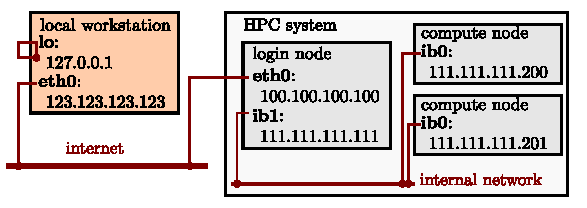
\includegraphics[width=0.9\textwidth]{figures/ipi-network.pdf}
\caption{\label{fig:network} A schematic representation of the network layout one 
typically finds when running \ipi and the clients on a HPC system and/or on a local workstation. } 
\end{figure}

Figure~\ref{fig:network} represents schematically a typical network layout
for a HPC system and a local workstation. When running \ipi locally on a 
workstation, one can use the loopback interface (that can be referred to as 
``localhost'' in the ``address'' field of both \ipi and the client) for communication.
When running both \ipi and the clients on a HPC cluster, one should work out which of the
the interfaces that are available on the node where the \ipi server runs are accessible from the
compute nodes. This requires some trial and error, and possibly setting the 
 ``address'' field dynamically from the job that launches \ipi. 
 For instance,
if one was running \ipi on the login node, and the clients on different compute nodes, as 
in Figure~\ref{fig:running}b, then on the HPC system described in Figure~\ref{fig:network} 
one should set the address to that of the \emph{ib1} interface -- $111.111.111.111$ in 
the example above. If instead \ipi was launched in a job script, then the submission script would
have to check for the IP address associated with the \emph{ib0} interface on the node
the job has been dispatched to, and set that address (e.g. $111.111.111.200$) in the inputs
of both \ipi and the clients that will be launched in the same (or separate) jobs.

Running \ipi on a separate workstation (Figure~\ref{fig:running}c) gives 
maximum flexibility, but is also trickier as one has to reach the 
internet from the compute nodes, that are typically not directly connected to it. 
We discuss this more advanced setup in the next paragraph.

\subsubsection{ssh tunnelling}

\label{ssh_sockets}

If \ipi is to be run in a distributed computing mode, then one should
make sure that the workstation on which the server will run is accessible from
the outside internet on the range of ports that one wants to use for
\ipi. There are ways to circumvent a firewall, but we will not discuss them
here, as the whole point of \ipi is that it can be run on a low-profile
PC whose security does not need to be critical. Typically arrangements
can be made to open up a range of ports for incoming connections. 

A more substantial problem -- as it depends on the physical layout
of the network rather than on software settings of the firewall --
is how to access the workstation from the compute nodes, which in most
cases do not have a network interface directly connected to the 
outside internet.

The problem can be solved by creating a ssh tunnel, i.e. an instance of
the ssh secure shell that will connect the compute node to the login node, 
and then forward all traffic that is directed to a designated port
on the compute node to the remote location that is running \ipi, passing
through the outbound network interface of the login node. 

In the example above, if \ipi{} is running on a local workstation, one should run:

\begin{code}
> ssh -f -N -L local_port:workstation:remote_port -2 login_node
\end{code}

\noindent from the job script that launches the client. 
For instance, with the network layout of Figure~\ref{fig:network}, 
and if the \ipi{} server is listening
on port 12345 of the \emph{eth0} interface, the tunnel should be created as:

\begin{code}
> ssh -f -N -L 54321:123.123.123.123:12345 -2 111.111.111.111
\end{code}

\noindent The client should then be configured to connect to \emph{localhost}
on port 54321. The connection with \ipi will be established through the tunnel,
and the data exchange can begin.

Note that, in order to be able to include the above commands in a script,
the login node and the compute nodes should be configured to allow 
password-less login within the HPC system. This can be achieved easily, and
does not entail significant security risks, since it only allows one to 
connect from one node to another within the local network.
To do so, you should log onto the HPC system, and create a pair 
of ssh keys (if this has not been done already, in which case an 
id\_rsa.pub file should be present in the user's \textasciitilde{}/.ssh/ directory) 
by issuing the command 

\begin{code}
> ssh-keygen -t rsa
\end{code}

\noindent The program will then prompt for a passphrase twice. Since we wish to have
use this in a job script where we will not be able to enter a password,
just hit enter twice. 

This should now have created two files in the directory \textasciitilde{}/.ssh,
id\_rsa and id\_rsa.pub. These should be readable only by you, so
use the following code to set up the correct file permissions:

\begin{code}
> chmod 600 ~/.ssh/id_rsa ~/.ssh/id_rsa.pub
\end{code}

\noindent Finally, copy the contents of the file id\_rsa.pub and append them
to the file authorized\_keys in the directory \textasciitilde{}/.ssh
of the user on the login node, which is typically shared among all
the nodes of a cluster and therefore allows password-less login 
from all of the compute nodes.


\chapter{Input reference}

\label{hierarchy}

This chapter gives a complete list of the tags that can be
specified in the xml input file, along with the hierarchy of objects.
Note that every xml input file must start with the root tag 
{}``\hyperref[SIMULATION]{simulation}''. 
See the accompanying {}``help.xml'' file in the {}``doc/help\_files'' directory
to see the recommended input file structure.

Each section of this chapter describes one of the major input classes
used in the \ipi initialization. These sections will start with some normal
text which describes the function of this class in detail.
After this the attributes of the tag will be listed, enclosed within
a frame for clarity.
Finally, the fields contained within the tag will be listed in alphabetical order,
possibly followed by their attributes.
\textbf{Attribute} names will be bold and 
\textbf{\underline{field}} names both bold and underlined.
\emph{\small Other supplementary information} will be in small font and italicized.

\subsection{SIMULATION}
\label{SIMULATION}
This is the top level class that deals with the running of the simulation, including holding the simulation specific properties such as the time step and outputting the data.
\paragraph{Fields}
 \begin{itemize}
\item {\bf \hyperref[FORCES]{force} }:
 Deals with the assigning of jobs to different driver codes, and collecting the data.
\paragraph{Attributes}
 \begin{itemize}
\item {\bf type}:
 Specifies which kind of force object is created
{\\ \bf DEFAULT: }'socket'
{\\ \bf OPTIONS: }'socket'
{\\ \bf DATA TYPE: }str
\end{itemize}
 
\paragraph{Fields}
 \begin{itemize}
\item {\bf interface}:
 Specifies the parameters for the socket interface.
\item {\bf parameters}:
 deprecated dictionary of initialization parameters. May be removed in the future.
{\\ \bf DEFAULT: }\{ \}
{\\ \bf DATA TYPE: }dict
\end{itemize}
 
\item {\bf trajectories}:
 A list of the allowed properties to print out the per-atom or per-bead trajectories of. Allowed values are ['positions', 'velocities', 'forces', 'kinetic\_cv', 'centroid'].
{\\ \bf DEFAULT: }[ ]
{\\ \bf DATA TYPE: }str
\paragraph{Attributes}
 \begin{itemize}
\item {\bf shape}:
 The shape of the array
{\\ \bf DEFAULT: }(0,)
{\\ \bf DATA TYPE: }tuple
\end{itemize}
 
\item {\bf \hyperref[ATOMS]{atoms} }:
 Deals with classical simulations.
\paragraph{Fields}
 \begin{itemize}
\item {\bf q}:
 The positions of the atoms, in the format [x1, y1, z1, x2, \ldots  ]
{\\ \bf DIMENSION: }length
{\\ \bf DEFAULT: }[ ]
{\\ \bf DATA TYPE: }float
\item {\bf p}:
 The momenta of the atoms, in the format [px1, py1, pz1, px2, \ldots  ]
{\\ \bf DIMENSION: }momentum
{\\ \bf DEFAULT: }[ ]
{\\ \bf DATA TYPE: }float
\item {\bf natoms}:
 The number of atoms
{\\ \bf DEFAULT: }0
{\\ \bf DATA TYPE: }int
\item {\bf names}:
 The names of the atoms, in the format [name1, name2, \ldots  ]
{\\ \bf DEFAULT: }[ ]
{\\ \bf DATA TYPE: }str
\item {\bf file\_units}:
 The units in which the lengths in the configuration file are given.
{\\ \bf DEFAULT: }''
{\\ \bf OPTIONS: }'', 'nanometer', 'angstrom', 'atomic\_unit'
{\\ \bf DATA TYPE: }str
\item {\bf from\_file}:
 Gives the name of the file from which the configurations are taken, if present.
{\\ \bf DEFAULT: }''
{\\ \bf DATA TYPE: }str
\item {\bf m}:
 The masses of the atoms, in the format [m1, m2, \ldots  ]
{\\ \bf DIMENSION: }mass
{\\ \bf DEFAULT: }[ ]
{\\ \bf DATA TYPE: }float
\item {\bf init\_temp}:
 The temperature at which the initial velocity distribution is taken, if applicable.
{\\ \bf DIMENSION: }temperature
{\\ \bf DEFAULT: }-1.0
{\\ \bf DATA TYPE: }float
\end{itemize}
 
\item {\bf step}:
 How many time steps have been done.
{\\ \bf DEFAULT: }0
{\\ \bf DATA TYPE: }int
\item {\bf initialize}:
 A dictionary giving the properties of the system that need to be initialized, and their initial values. The allowed keywords are ['velocities']. The initial value of 'velocities' corresponds to the temperature to initialise the velocity distribution from. If 0, then the sysytem temperature is used.
{\\ \bf DEFAULT: }\{ \}
{\\ \bf DATA TYPE: }dict
\item {\bf properties}:
 A list of the properties that will be printed in the properties output file. See the manual for a full list of acceptable names.
{\\ \bf DEFAULT: }[ ]
{\\ \bf DATA TYPE: }str
\paragraph{Attributes}
 \begin{itemize}
\item {\bf shape}:
 The shape of the array
{\\ \bf DEFAULT: }(0,)
{\\ \bf DATA TYPE: }tuple
\end{itemize}
 
\item {\bf \hyperref[BEADS]{beads} }:
 Deals with path integral simulations.
\paragraph{Fields}
 \begin{itemize}
\item {\bf q}:
 The positions of the atoms, in the format [x1, y1, z1, x2, \ldots  ]
{\\ \bf DIMENSION: }length
{\\ \bf DEFAULT: }[ ]
{\\ \bf DATA TYPE: }float
\item {\bf p}:
 The momenta of the atoms, in the format [px1, py1, pz1, px2, \ldots  ]
{\\ \bf DIMENSION: }momentum
{\\ \bf DEFAULT: }[ ]
{\\ \bf DATA TYPE: }float
\item {\bf natoms}:
 The number of atoms
{\\ \bf DEFAULT: }0
{\\ \bf DATA TYPE: }int
\item {\bf start\_centroid}:
 An atoms object from which the centroid coordinates can be initialized
\item {\bf nbeads}:
 The number of beads
{\\ \bf DATA TYPE: }int
\item {\bf m}:
 The masses of the atoms, in the format [m1, m2, \ldots  ]
{\\ \bf DIMENSION: }mass
{\\ \bf DEFAULT: }[ ]
{\\ \bf DATA TYPE: }float
\item {\bf init\_temp}:
 The temperature at which the initial velocity distribution is taken, if applicable.
{\\ \bf DIMENSION: }temperature
{\\ \bf DEFAULT: }-1.0
{\\ \bf DATA TYPE: }float
\item {\bf names}:
 The names of the atoms, in the format [name1, name2, \ldots  ]
{\\ \bf DEFAULT: }[ ]
{\\ \bf DATA TYPE: }str
\end{itemize}
 
\item {\bf total\_steps}:
 The total number of steps that will be done.
{\\ \bf DEFAULT: }1000
{\\ \bf DATA TYPE: }int
\item {\bf prefix}:
 A string that will be the prefix for all the output file names.
{\\ \bf DEFAULT: }'prefix'
{\\ \bf DATA TYPE: }str
\item {\bf fd\_delta}:
 The parameter used in the finite difference differentiation in the calculation of the scaled path velocity estimator.
{\\ \bf DEFAULT: }0.0
{\\ \bf DATA TYPE: }float
\item {\bf \hyperref[CELL]{cell} }:
 Deals with the cell parameters, and stores their momenta in flexible cell calculations.
\paragraph{Attributes}
 \begin{itemize}
\item {\bf flexible}:
 Whether the cell parameters can change during the simulation.
{\\ \bf DEFAULT: }False
{\\ \bf DATA TYPE: }bool
\end{itemize}
 
\paragraph{Fields}
 \begin{itemize}
\item {\bf from\_file}:
 A file from which to take the cell parameters from.
{\\ \bf DEFAULT: }''
{\\ \bf DATA TYPE: }str
\item {\bf p}:
 The cell 'momenta' matrix, used in constant pressure simulations.
{\\ \bf DIMENSION: }momentum
{\\ \bf DEFAULT: }
      [[ 0.  0.  0.]
       [ 0.  0.  0.]
       [ 0.  0.  0.]]
{\\ \bf DATA TYPE: }float
\item {\bf init\_temp}:
 The temperature at which the initial velocity distribution is taken, if applicable.
{\\ \bf DIMENSION: }temperature
{\\ \bf DEFAULT: }-1.0
{\\ \bf DATA TYPE: }float
\item {\bf P}:
 The scalar cell 'momentum', used in constant pressure simulations.
{\\ \bf DIMENSION: }momentum
{\\ \bf DEFAULT: }0.0
{\\ \bf DATA TYPE: }float
\item {\bf file\_units}:
 The units in which the lengths in the configuration file are given.
{\\ \bf DEFAULT: }''
{\\ \bf OPTIONS: }'', 'nanometer', 'angstrom', 'atomic\_unit'
{\\ \bf DATA TYPE: }str
\item {\bf h}:
 The cell vector matrix
{\\ \bf DIMENSION: }length
{\\ \bf DEFAULT: }
      [[ 0.  0.  0.]
       [ 0.  0.  0.]
       [ 0.  0.  0.]]
{\\ \bf DATA TYPE: }float
\item {\bf h0}:
 The reference cell vector matrix. Defined as the unstressed equilibrium cell.
{\\ \bf DIMENSION: }length
{\\ \bf DEFAULT: }
      [[ 0.  0.  0.]
       [ 0.  0.  0.]
       [ 0.  0.  0.]]
{\\ \bf DATA TYPE: }float
\item {\bf m}:
 The 'mass' of the cell, used in constant pressure simulations.
{\\ \bf DIMENSION: }mass
{\\ \bf DEFAULT: }0.0
{\\ \bf DATA TYPE: }float
\end{itemize}
 
\item {\bf stride}:
 Dictionary holding the number of steps between printing the different kinds of files. The allowed keywords are ['checkpoint', 'properties', 'progress', 'trajectory', centroid']
{\\ \bf DEFAULT: }\{ \}
{\\ \bf DATA TYPE: }dict
\item {\bf traj\_format}:
 The file format for the output file. Allowed keywords are ['pdb', 'xyz'].
{\\ \bf DEFAULT: }'pdb'
{\\ \bf DATA TYPE: }str
\item {\bf \hyperref[RANDOM]{prng} }:
 Deals with the pseudo-random number generator.
\paragraph{Fields}
 \begin{itemize}
\item {\bf has\_gauss}:
 Determines whether there is a stored gaussian number or not. A value of 0 means there is none stored.
{\\ \bf DEFAULT: }0
{\\ \bf DATA TYPE: }int
\item {\bf state}:
 Gives the state vector for the random number generator. Avoid directly modifying this unless you are very familiar with the inner workings of the algorithm used.
{\\ \bf DEFAULT: }[ ]
{\\ \bf DATA TYPE: }uint64
\item {\bf seed}:
 This is the seed number used to generate the initial state of the random number generator.
{\\ \bf DEFAULT: }123456
{\\ \bf DATA TYPE: }int
\item {\bf set\_pos}:
 Gives the position in the state array that the random number generator is reading from.
{\\ \bf DEFAULT: }0
{\\ \bf DATA TYPE: }int
\item {\bf gauss}:
 The stored Gaussian number.
{\\ \bf DEFAULT: }0.0
{\\ \bf DATA TYPE: }float
\end{itemize}
 
\item {\bf \hyperref[ENSEMBLE]{ensemble} }:
 Holds all the information that is ensemble specific, such as the temperature and the external pressure, and the thermostats and barostats that control it.
\paragraph{Attributes}
 \begin{itemize}
\item {\bf type}:
 The ensemble that will be sampled during the simulation.
{\\ \bf DEFAULT: }'nve'
{\\ \bf OPTIONS: }'nve', 'nvt', 'npt', 'nst'
{\\ \bf DATA TYPE: }str
\end{itemize}
 
\paragraph{Fields}
 \begin{itemize}
\item {\bf stress}:
 The external stress.
{\\ \bf DIMENSION: }pressure
{\\ \bf DEFAULT: }
      [[ 1.  0.  0.]
       [ 0.  1.  0.]
       [ 0.  0.  1.]]
{\\ \bf DATA TYPE: }float
\item {\bf barostat}:
 Simulates an external pressure bath to keep the pressure or stress at the external values.
\item {\bf thermostat}:
 The thermostat for the atoms, keeps the atom velocity distribution at the correct temperature.
\item {\bf timestep}:
 The time step.
{\\ \bf DIMENSION: }time
{\\ \bf DEFAULT: }'1.0'
{\\ \bf DATA TYPE: }float
\item {\bf pressure}:
 The external pressure.
{\\ \bf DIMENSION: }pressure
{\\ \bf DEFAULT: }'1.0'
{\\ \bf DATA TYPE: }float
\item {\bf fixcom}:
 This describes whether the centre of mass of the particles is fixed.
{\\ \bf DEFAULT: }False
{\\ \bf DATA TYPE: }bool
\item {\bf temperature}:
 The temperature of the system.
{\\ \bf DIMENSION: }temperature
{\\ \bf DEFAULT: }1.0
{\\ \bf DATA TYPE: }float
\end{itemize}
 
\end{itemize}
 

\input{input_docs/paratemp}
\input{input_docs/forcefield}
\input{input_docs/ffsocket}
\input{input_docs/system}
\input{input_docs/initializer}
\input{input_docs/init_file}
\input{input_docs/init_pos}
\input{input_docs/init_mom}
\input{input_docs/init_vel}
\input{input_docs/init_lab}
\input{input_docs/init_mass}
\input{input_docs/init_cell}
\input{input_docs/init_therm}
\section{ENSEMBLE}
\label{ENSEMBLE}
Holds all the information that is ensemble specific, such as the temperature and the external pressure, and the thermostats and barostats that control it.
\paragraph{Attributes}
 \begin{itemize}
\item {\bf type}:
 The ensemble that will be sampled during the simulation.
{\\ \bf DEFAULT: }'nve'
{\\ \bf OPTIONS: }'nve', 'nvt', 'npt', 'nst'
{\\ \bf DATA TYPE: }str
\end{itemize}
 
\paragraph{Fields}
 \begin{itemize}
\item {\bf stress}:
 The external stress.
{\\ \bf DIMENSION: }pressure
{\\ \bf DEFAULT: }
      [[ 1.  0.  0.]
       [ 0.  1.  0.]
       [ 0.  0.  1.]]
{\\ \bf DATA TYPE: }float
\paragraph{Attributes}
 \begin{itemize}
\item {\bf shape}:
 The shape of the array.
{\\ \bf DEFAULT: }(0,)
{\\ \bf DATA TYPE: }tuple
\end{itemize}
 
\item {\bf \hyperref[BAROSTAT]{barostat} }:
 Simulates an external pressure bath to keep the pressure or stress at the external values.
\paragraph{Attributes}
 \begin{itemize}
\item {\bf kind}:
 The type of barostat. 'Rigid' gives a barostat that keeps the internal pressure constant by allowing cell volume changes, whereas flexible allows the shape of the cell to fluctuate too.
{\\ \bf DEFAULT: }'rigid'
{\\ \bf OPTIONS: }'rigid', 'flexible'
{\\ \bf DATA TYPE: }str
\end{itemize}
 
\item {\bf \hyperref[THERMOSTATS]{thermostat} }:
 The thermostat for the atoms, keeps the atom velocity distribution at the correct temperature.
\paragraph{Attributes}
 \begin{itemize}
\item {\bf kind}:
 The style of thermostatting.
{\\ \bf DEFAULT: }'langevin'
{\\ \bf OPTIONS: }'langevin', 'svr', 'pile\_l', 'pile\_g', 'gle', 'nm\_gle'
{\\ \bf DATA TYPE: }str
\end{itemize}
 
\item {\bf timestep}:
 The time step.
{\\ \bf DIMENSION: }time
{\\ \bf DEFAULT: }'1.0'
{\\ \bf DATA TYPE: }float
\item {\bf pressure}:
 The external pressure.
{\\ \bf DIMENSION: }pressure
{\\ \bf DEFAULT: }'1.0'
{\\ \bf DATA TYPE: }float
\item {\bf fixcom}:
 This describes whether the centre of mass of the particles is fixed.
{\\ \bf DEFAULT: }False
{\\ \bf DATA TYPE: }bool
\item {\bf temperature}:
 The temperature of the system.
{\\ \bf DIMENSION: }temperature
{\\ \bf DEFAULT: }1.0
{\\ \bf DATA TYPE: }float
\end{itemize}
 

\subsection{FORCES}
\label{FORCES}
Deals with the assigning of jobs to different driver codes, and collecting the data.
\paragraph{Attributes}
 \begin{itemize}
\item {\bf type}:
 Specifies which kind of force object is created
{\\ \bf DEFAULT: }'socket'
{\\ \bf OPTIONS: }'socket'
{\\ \bf DATA TYPE: }str
\end{itemize}
 
\paragraph{Fields}
 \begin{itemize}
\item {\bf \hyperref[INTERFACE]{interface} }:
 Specifies the parameters for the socket interface.
\paragraph{Attributes}
 \begin{itemize}
\item {\bf mode}:
 Specifies whether the driver interface will listen onto a internet socket [inet] or onto a unix socket [unix]
{\\ \bf DEFAULT: }'inet'
{\\ \bf OPTIONS: }'unix', 'inet'
{\\ \bf DATA TYPE: }str
\end{itemize}
 
\paragraph{Fields}
 \begin{itemize}
\item {\bf latency}:
 This gives the number of seconds between each check for new clients
{\\ \bf DEFAULT: }0.001
{\\ \bf DATA TYPE: }float
\item {\bf slots}:
 This gives the number of client codes that queue at any one time
{\\ \bf DEFAULT: }4
{\\ \bf DATA TYPE: }int
\item {\bf port}:
 This gives the port number that defines the socket
{\\ \bf DEFAULT: }31415
{\\ \bf DATA TYPE: }int
\item {\bf timeout}:
 This gives the number of seconds before assuming a calculation has died. If 0 there is no timeout.
{\\ \bf DEFAULT: }0.0
{\\ \bf DATA TYPE: }float
\item {\bf address}:
 This gives the server address that the socket will run on
{\\ \bf DEFAULT: }'localhost'
{\\ \bf DATA TYPE: }str
\end{itemize}
 
\item {\bf parameters}:
 deprecated dictionary of initialization parameters. May be removed in the future.
{\\ \bf DEFAULT: }\{ \}
{\\ \bf DATA TYPE: }dict
\end{itemize}
 

\input{input_docs/forcecomponent}
\subsection{CELL}
\label{CELL}
Deals with the cell parameters, and stores their momenta in flexible cell calculations.
\paragraph{Attributes}
 \begin{itemize}
\item {\bf flexible}:
 Whether the cell parameters can change during the simulation.
{\\ \bf DEFAULT: }False
{\\ \bf DATA TYPE: }bool
\end{itemize}
 
\paragraph{Fields}
 \begin{itemize}
\item {\bf from\_file}:
 A file from which to take the cell parameters from.
{\\ \bf DEFAULT: }''
{\\ \bf DATA TYPE: }str
\item {\bf p}:
 The cell 'momenta' matrix, used in constant pressure simulations.
{\\ \bf DIMENSION: }momentum
{\\ \bf DEFAULT: }
      [[ 0.  0.  0.]
       [ 0.  0.  0.]
       [ 0.  0.  0.]]
{\\ \bf DATA TYPE: }float
\paragraph{Attributes}
 \begin{itemize}
\item {\bf shape}:
 The shape of the array
{\\ \bf DEFAULT: }(0,)
{\\ \bf DATA TYPE: }tuple
\end{itemize}
 
\item {\bf init\_temp}:
 The temperature at which the initial velocity distribution is taken, if applicable.
{\\ \bf DIMENSION: }temperature
{\\ \bf DEFAULT: }-1.0
{\\ \bf DATA TYPE: }float
\item {\bf P}:
 The scalar cell 'momentum', used in constant pressure simulations.
{\\ \bf DIMENSION: }momentum
{\\ \bf DEFAULT: }0.0
{\\ \bf DATA TYPE: }float
\item {\bf file\_units}:
 The units in which the lengths in the configuration file are given.
{\\ \bf DEFAULT: }''
{\\ \bf OPTIONS: }'', 'nanometer', 'angstrom', 'atomic\_unit'
{\\ \bf DATA TYPE: }str
\item {\bf h}:
 The cell vector matrix
{\\ \bf DIMENSION: }length
{\\ \bf DEFAULT: }
      [[ 0.  0.  0.]
       [ 0.  0.  0.]
       [ 0.  0.  0.]]
{\\ \bf DATA TYPE: }float
\paragraph{Attributes}
 \begin{itemize}
\item {\bf shape}:
 The shape of the array
{\\ \bf DEFAULT: }(0,)
{\\ \bf DATA TYPE: }tuple
\end{itemize}
 
\item {\bf h0}:
 The reference cell vector matrix. Defined as the unstressed equilibrium cell.
{\\ \bf DIMENSION: }length
{\\ \bf DEFAULT: }
      [[ 0.  0.  0.]
       [ 0.  0.  0.]
       [ 0.  0.  0.]]
{\\ \bf DATA TYPE: }float
\paragraph{Attributes}
 \begin{itemize}
\item {\bf shape}:
 The shape of the array
{\\ \bf DEFAULT: }(0,)
{\\ \bf DATA TYPE: }tuple
\end{itemize}
 
\item {\bf m}:
 The 'mass' of the cell, used in constant pressure simulations.
{\\ \bf DIMENSION: }mass
{\\ \bf DEFAULT: }0.0
{\\ \bf DATA TYPE: }float
\end{itemize}
 

\section{BEADS}
\label{BEADS}
Deals with path integral simulations.
\paragraph{Fields}
 \begin{itemize}
\item {\bf q}:
 The positions of the atoms, in the format [x1, y1, z1, x2, \ldots  ]
{\\ \bf DIMENSION: }length
{\\ \bf DEFAULT: }[ ]
{\\ \bf DATA TYPE: }float
\paragraph{Attributes}
 \begin{itemize}
\item {\bf shape}:
 The shape of the array
{\\ \bf DEFAULT: }(0,)
{\\ \bf DATA TYPE: }tuple
\end{itemize}
 
\item {\bf p}:
 The momenta of the atoms, in the format [px1, py1, pz1, px2, \ldots  ]
{\\ \bf DIMENSION: }momentum
{\\ \bf DEFAULT: }[ ]
{\\ \bf DATA TYPE: }float
\paragraph{Attributes}
 \begin{itemize}
\item {\bf shape}:
 The shape of the array
{\\ \bf DEFAULT: }(0,)
{\\ \bf DATA TYPE: }tuple
\end{itemize}
 
\item {\bf natoms}:
 The number of atoms
{\\ \bf DEFAULT: }0
{\\ \bf DATA TYPE: }int
\item {\bf \hyperref[ATOMS]{start\_centroid} }:
 An atoms object from which the centroid coordinates can be initialized
\item {\bf nbeads}:
 The number of beads
{\\ \bf DATA TYPE: }int
\item {\bf m}:
 The masses of the atoms, in the format [m1, m2, \ldots  ]
{\\ \bf DIMENSION: }mass
{\\ \bf DEFAULT: }[ ]
{\\ \bf DATA TYPE: }float
\paragraph{Attributes}
 \begin{itemize}
\item {\bf shape}:
 The shape of the array
{\\ \bf DEFAULT: }(0,)
{\\ \bf DATA TYPE: }tuple
\end{itemize}
 
\item {\bf init\_temp}:
 The temperature at which the initial velocity distribution is taken, if applicable.
{\\ \bf DIMENSION: }temperature
{\\ \bf DEFAULT: }-1.0
{\\ \bf DATA TYPE: }float
\item {\bf names}:
 The names of the atoms, in the format [name1, name2, \ldots  ]
{\\ \bf DEFAULT: }[ ]
{\\ \bf DATA TYPE: }str
\paragraph{Attributes}
 \begin{itemize}
\item {\bf shape}:
 The shape of the array
{\\ \bf DEFAULT: }(0,)
{\\ \bf DATA TYPE: }tuple
\end{itemize}
 
\end{itemize}
 

\section{ATOMS}
\label{ATOMS}
Deals with single replicas of the system or classical simulations.
\paragraph{Fields}
 \begin{itemize}
\item {\bf q}:
 The positions of the atoms, in the format [x1, y1, z1, x2, \ldots  ]
{\\ \bf DIMENSION: }length
{\\ \bf DEFAULT: }[ ]
{\\ \bf DATA TYPE: }float
\paragraph{Attributes}
 \begin{itemize}
\item {\bf shape}:
 The shape of the array
{\\ \bf DEFAULT: }(0,)
{\\ \bf DATA TYPE: }tuple
\end{itemize}
 
\item {\bf p}:
 The momenta of the atoms, in the format [px1, py1, pz1, px2, \ldots  ]
{\\ \bf DIMENSION: }momentum
{\\ \bf DEFAULT: }[ ]
{\\ \bf DATA TYPE: }float
\paragraph{Attributes}
 \begin{itemize}
\item {\bf shape}:
 The shape of the array
{\\ \bf DEFAULT: }(0,)
{\\ \bf DATA TYPE: }tuple
\end{itemize}
 
\item {\bf natoms}:
 The number of atoms
{\\ \bf DEFAULT: }0
{\\ \bf DATA TYPE: }int
\item {\bf names}:
 The names of the atoms, in the format [name1, name2, \ldots  ]
{\\ \bf DEFAULT: }[ ]
{\\ \bf DATA TYPE: }str
\paragraph{Attributes}
 \begin{itemize}
\item {\bf shape}:
 The shape of the array
{\\ \bf DEFAULT: }(0,)
{\\ \bf DATA TYPE: }tuple
\end{itemize}
 
\item {\bf file\_units}:
 The units in which the lengths in the configuration file are given.
{\\ \bf DEFAULT: }''
{\\ \bf OPTIONS: }'', 'nanometer', 'angstrom', 'atomic\_unit'
{\\ \bf DATA TYPE: }str
\item {\bf from\_file}:
 Gives the name of the file from which the configurations are taken, if present.
{\\ \bf DEFAULT: }''
{\\ \bf DATA TYPE: }str
\item {\bf m}:
 The masses of the atoms, in the format [m1, m2, \ldots  ]
{\\ \bf DIMENSION: }mass
{\\ \bf DEFAULT: }[ ]
{\\ \bf DATA TYPE: }float
\paragraph{Attributes}
 \begin{itemize}
\item {\bf shape}:
 The shape of the array
{\\ \bf DEFAULT: }(0,)
{\\ \bf DATA TYPE: }tuple
\end{itemize}
 
\item {\bf init\_temp}:
 The temperature at which the initial velocity distribution is taken, if applicable.
{\\ \bf DIMENSION: }temperature
{\\ \bf DEFAULT: }-1.0
{\\ \bf DATA TYPE: }float
\end{itemize}
 

\input{input_docs/normal_modes}
\subsection{BAROSTAT}
\label{BAROSTAT}
Simulates an external pressure bath to keep the pressure or stress at the external values.
\paragraph{Attributes}
 \begin{itemize}
\item {\bf kind}:
 The type of barostat.
{\\ \bf DEFAULT: }'rigid'
{\\ \bf OPTIONS: }'rigid', 'flexible'
{\\ \bf DATA TYPE: }str
\end{itemize}
 
\paragraph{Fields}
 \begin{itemize}
\item {\bf \hyperref[THERMOSTATS]{thermostat} }:
 The thermostat for the cell. Keeps the cell velocity distribution at the correct temperature.
\paragraph{Attributes}
 \begin{itemize}
\item {\bf kind}:
 The style of thermostatting.
{\\ \bf DEFAULT: }'langevin'
{\\ \bf OPTIONS: }'langevin', 'svr', 'pile\_l', 'pile\_g', 'gle', 'nm\_gle'
{\\ \bf DATA TYPE: }str
\end{itemize}
 
\paragraph{Fields}
 \begin{itemize}
\item {\bf A}:
 The friction matrix for GLE thermostats.
{\\ \bf DIMENSION: }frequency
{\\ \bf DEFAULT: }[ ]
{\\ \bf DATA TYPE: }float
\item {\bf tau}:
 The target temperature for the thermostat.
{\\ \bf DIMENSION: }temperature
{\\ \bf DEFAULT: }0.0
{\\ \bf DATA TYPE: }float
\item {\bf C}:
 The covariance matrix for GLE thermostats.
{\\ \bf DIMENSION: }temperature
{\\ \bf DEFAULT: }[ ]
{\\ \bf DATA TYPE: }float
\item {\bf s}:
 Input values for the additional momenta in GLE.
{\\ \bf DIMENSION: }ms-momentum
{\\ \bf DEFAULT: }[ ]
{\\ \bf DATA TYPE: }float
\item {\bf ethermo}:
 The initial value of the thermostat energy. Only useful in restarts to guarantee continuity of the conserved quantity. 
{\\ \bf DIMENSION: }energy
{\\ \bf DEFAULT: }0.0
{\\ \bf DATA TYPE: }float
\end{itemize}
 
\end{itemize}
 

\section{THERMOSTATS}
\label{THERMOSTATS}
Simulates an external heat bath to keep the velocity distribution at the correct temperature.
\paragraph{Attributes}
 \begin{itemize}
\item {\bf kind}:
 The style of thermostatting. 'langevin' specifies a white noise langevin equation to be attached to the cartesian representation of the momenta. 'svr' attaches a velocity rescaling thermostat to the cartesian representation of the momenta. Both 'pile\_l' and 'pile\_g' attaches a white noise langevin thermostat to the normal mode representation, with 'pile\_l' attaching a local langevin thermostat to the centroid mode and 'pile\_g' instead attaching a global velocity rescaling thermostat. 'gle' attaches a coloured noise langevin thermostat to the cartesian representation of the momenta, and 'nm\_gle' attaches a coloured noise langevin thermostat to the normal mode representation of the momenta.
{\\ \bf DEFAULT: }'langevin'
{\\ \bf OPTIONS: }'langevin', 'svr', 'pile\_l', 'pile\_g', 'gle', 'nm\_gle', 'nm\_gle\_g'
{\\ \bf DATA TYPE: }str
\end{itemize}
 
\paragraph{Fields}
 \begin{itemize}
\item {\bf A}:
 The friction matrix for GLE thermostats.
{\\ \bf DIMENSION: }frequency
{\\ \bf DEFAULT: }[ ]
{\\ \bf DATA TYPE: }float
\paragraph{Attributes}
 \begin{itemize}
\item {\bf shape}:
 The shape of the array.
{\\ \bf DEFAULT: }(0,)
{\\ \bf DATA TYPE: }tuple
\end{itemize}
 
\item {\bf tau}:
 The friction coefficient for white noise thermostats.
{\\ \bf DIMENSION: }temperature
{\\ \bf DEFAULT: }0.0
{\\ \bf DATA TYPE: }float
\item {\bf C}:
 The covariance matrix for GLE thermostats.
{\\ \bf DIMENSION: }temperature
{\\ \bf DEFAULT: }[ ]
{\\ \bf DATA TYPE: }float
\paragraph{Attributes}
 \begin{itemize}
\item {\bf shape}:
 The shape of the array.
{\\ \bf DEFAULT: }(0,)
{\\ \bf DATA TYPE: }tuple
\end{itemize}
 
\item {\bf s}:
 Input values for the additional momenta in GLE.
{\\ \bf DIMENSION: }ms-momentum
{\\ \bf DEFAULT: }[ ]
{\\ \bf DATA TYPE: }float
\paragraph{Attributes}
 \begin{itemize}
\item {\bf shape}:
 The shape of the array.
{\\ \bf DEFAULT: }(0,)
{\\ \bf DATA TYPE: }tuple
\end{itemize}
 
\item {\bf ethermo}:
 The initial value of the thermostat energy. Used when the simulation is restarted to guarantee continuity of the conserved quantity.
{\\ \bf DIMENSION: }energy
{\\ \bf DEFAULT: }0.0
{\\ \bf DATA TYPE: }float
\end{itemize}
 

\section{RANDOM}
\label{RANDOM}
Deals with the pseudo-random number generator.
\paragraph{Fields}
 \begin{itemize}
\item {\bf has\_gauss}:
 Determines whether there is a stored gaussian number or not. A value of 0 means there is none stored.
{\\ \bf DEFAULT: }0
{\\ \bf DATA TYPE: }int
\item {\bf state}:
 Gives the state vector for the random number generator. Avoid directly modifying this unless you are very familiar with the inner workings of the algorithm used.
{\\ \bf DEFAULT: }[ ]
{\\ \bf DATA TYPE: }uint64
\paragraph{Attributes}
 \begin{itemize}
\item {\bf shape}:
 The shape of the array.
{\\ \bf DEFAULT: }(0,)
{\\ \bf DATA TYPE: }tuple
\end{itemize}
 
\item {\bf seed}:
 This is the seed number used to generate the initial state of the random number generator.
{\\ \bf DEFAULT: }123456
{\\ \bf DATA TYPE: }int
\item {\bf set\_pos}:
 Gives the position in the state array that the random number generator is reading from.
{\\ \bf DEFAULT: }0
{\\ \bf DATA TYPE: }int
\item {\bf gauss}:
 The stored Gaussian number.
{\\ \bf DEFAULT: }0.0
{\\ \bf DATA TYPE: }float
\end{itemize}
 

\input{input_docs/output}
\input{input_docs/checkpoint}
\input{input_docs/properties}
\input{input_docs/trajectory}

\chapter{A simple tutorial}

\label{tutorial}

Here we give a simple step-by-step guide through an example
simulation, exploring
some of the more generally useful options that \ipi offers and making
no assumptions of previous experience of this code or other MD codes.
Excerpts from the relevant input files are reproduced here, for explanation
purposes, but to get the most out of this tutorial the user is strongly encouraged
to work through it themselves. For this purpose, the input files
have been included with the \ipi distribution, in the {}``test/tutorial''
directory.

The chosen problem is that of a small \emph{NPT} simulation of para-hydrogen, 
using the Silvera-Goldman potential \cite{silv-gold78jcp}. 
We will take (\(N\),\(P\),\(T\)) = (108, 0, 25 K).

\section{Part 1 - \emph{NVT} Equilibration run}

\label{part1}

\subsection{Client code}

Let us now consider the problem of how to use \ipi to run a \emph{NPT}
simulation of para-hydrogen. The first thing that is required is a
client code that is capable of calculating the potential interactions
of para-hydrogen molecules. Fortunately, one of the client codes distributed
with \ipi has an appropriate empirical potential already hard-coded
into it, and
so all that is required is to create the {}``driver.x'' file in
the {}``drivers'' directory, using the UNIX utility make.

This client code can be used for several different problems
(see \ref{driver.x}), some of which
are explored in the {}``examples'' directory, but for the current problem
we will use the Silvera-Goldman potential with a cut-off radius
of 15 \(a_0\). This is run using the following command:

\begin{code}
> ./driver.x -m sg -h localhost -o 15 -p 31415
\end{code}

The option {}``-m'' is followed by the empirical potential required,
in this case we use {}``sg'' for Silvera-Goldman, 
{}``-h localhost'' sets up the client hostname
as {}``localhost'', {}``-o 15'' sets the cut-off to 15 \(a_0\), 
and {}``-p 31415'' sets the port number to 31415. 

Note that usually this step will require setting up appropriate
client code input files, possibly for an \emph{ab initio} electronic
structure code, and so is generally a more involved process. Refer
to \ref{runningclients}, and the documentation of the appropriate
client code, for more details on how to do this step.


\subsection{Creating the xml input file}

Now that the client code is ready, an appropriate xml input file needs
to be created from which the host server and the simulation data can
be initialized. Here, we will go step by step through the creation
of a minimal input file for a simple \emph{NVT} equilibration run. Note that
the working final version is held within the {}``tutorial-1'' directory
for reference.

Firstly, when reading the input file the \ipi xml functions look
for a {}``simulation''
tag as a sign to start reading data. For those familiar with xml jargon,
we have defined {}``\hyperref[SIMULATION]{simulation}'' as the 
root tag, so all the input data read in must start and end with a 
{}``\hyperref[SIMULATION]{simulation}'' tag, as show below:

\begin{code}
<simulation>
   Input data here...
</simulation>
\end{code}

xml syntax requires a set of hierarchially nested tags, each of which
contain data and/or more tags. Also, \ipi itself requires certain
tags to be present, and keeps track of which tags are supposed to
be where. More information about which tags are available can be found
in \ref{hierarchy}, more information on xml syntax can be found in
\ref{ifilestructure}, and possible errors which can occur if the
input file is not well formed can be found in \ref{trouble}. 

For the sake of this first tutorial however, we will simply discuss the
those tags which are needed for a single \emph{NVT} equilibration run.
The most important tags are {}``\hyperref[INITIALIZER]{initialize}'', 
{}``\hyperref[ENSEMBLE]{ensemble}'', 
{}``total\_steps'' and {}``\hyperref[FORCES]{forces}''.
These correspond to the tag to initialize the atom configurations,
the tag to define the appropriate ensemble,
the tag to set the length of the simulation and the tag to specify the 
client code respectively.
We will also discuss {}``\hyperref[OUTPUTS]{output}'', 
which is used to define what output data
is generated by the code.

At this point then, the input file looks like:

\begin{code}
<simulation>
   <total_steps>
      ...
   </total_steps>
   <initialize>
      ...
   </initialize>
   <forces>
      ...
   </forces>
   <ensemble>
      ...
   </ensemble>
   <output>
      ...
   </output>
</simulation>
\end{code}

\subsubsection{Initializing the configurations}

Now let us consider each of these tags in turn. Firstly, 
{}``\hyperref[INITIALIZER]{initialize}''.
As the name suggests, this initializes the state of the system, so
this is where we will specify the atom positions and the cell
parameters. Firstly, this takes an attribute which specifies the number
of replicas of the system, called {}``nbeads''. An attribute is
a particular type of xml syntax designed to specify a single bit of
data, and has the following syntax:

\begin{code}
<initialize nbeads='4'>
   ...
</initialize>
\end{code}

Note that an attribute forms part of the opening tag, and that the
value being assigned to it is held within quotation marks. In this
case, we have set the number of replicas, or beads, to 4.

Next, we must specify the atomic configuration. Rather than initialize
the atom positions manually, we will instead use a separate configuration 
file for this purpose.
Here we will discuss two of the input formats that are compatible
with \ipi, xyz files and pdb files.

Note that, for the sake of this tutorial, we have 
included valid xyz and pdb input
files in the {}``tutorial-1'' directory called {}``our\_ref.xyz''
and {}``our\_ref.pdb'' respectively.

The xyz format is the simplest input format
for a configuration file that \ipi accepts, and has the following
syntax:

\begin{code}
natoms
# COMMENT LINE: PUT TITLE OF FILE HERE
atom1   x1  y1  z1
atom2   x2  y2  z2
...
\end{code}
where {}``natoms'' is replaced by an integer giving the total number
of atoms, in this case 108, atom1 is a label for atom 1, in this case
H2 (since we are simulating para-hydrogen), and (x1, y1, z1) are the
x, y and z components of atom 1 respectively. 

Note that we are treating the para-hydrogen molecules isotropically here,
i.e. as spherical psuedo-atoms.
For the current system this is a good approximation, since at 
the state point under consideration every molecule is in its 
rotational ground state. For further details on this potential,
and a demonstration of its application to quantum dynamics, see
\cite{silv-gold78jcp} and \cite{mill-mano05jcp}.

Other than its simplicity, the main advantage of this type of file
is that it is free-formatted, and so there is no set precision
to which each value must be written. This greatly simplifies
both reading and writing these files.

The other file format that we can use is the pdb format. This
has the following structure:

\begin{code}
TITLE insert title here...
CRYST1        a        b        c      A      B      C P 1           1
ATOM      1   n1   1     1          x1      y1      z1  0.00  0.00             0
ATOM      2   n2   1     1          x2      y2      z2  0.00  0.00             0
...
\end{code}
where a, b and c are the cell vector lengths, A, B and C are the angles between
them, n1 and n2 are the labels for atoms 1 and 2, and (x1, y1, z1)
and (x2, y2, z2) give the position vectors of atoms 1 and 2. 

Note that this is
fixed-formatted, so the number of spaces matters. Essentially, the
above format needs to be copied verbatim, using the same column
widths and all the same keywords. For an exact specification
of the file format (of which only a subset is implemented 
with \ipi) see
\url{http://deposit.rcsb.org/adit/docs/pdb_atom_format.html}.

Here we will show how to specify the xml input file
in both of these cases, assuming that the user has already
created the configuration file themselves.
Note that these file formats can be read by
visualization programs such as VMD, and so it is generally advised 
when making your own input files to
use such software to make sure that the configuration is as expected.

To use a configuration file the {}``\hyperref[INITFILE]{file}'' tag in 
{}``\hyperref[INITIALIZER]{initialize}'' should be used.
This will take an input file with a given name and use it to initialize
all relevant data. Both of these formats have the atom
positions and labels, so this will initialize the positions, labels
and masses of all the particles in the system, with the masses being
implicitly set based on the atom label. The pdb configuration file
will also be used to set the cell parameters.

Let us take these two file types in turn, and form the appropriate
input sections. First, the xyz file. 
There are two attributes which are 
relevant to the {}``\hyperref[INITFILE]{file}'' tag
for our current problem, {}``mode'' and {}``units''.
{}``mode'' is used to describe what kind of data is being used to
initialize from, and so in this case will be {}``xyz''.
{}``units'' specifies which units the file is given in, and
so in this case is given by {}``angstrom'', which are the
standard units of both xyz and pdb files. 
Note that if no units are specified then atomic units are assumed.
For more information on the \ipi unit conversion libraries, 
and the available units, see \ref{inputunits}.

This then gives:

\begin{code}
<initialize nbeads='4'>
   <file mode='xyz' units='angstrom'> our_ref.xyz </file>
   ...
</initialize>
\end{code}

In this case, since the cell parameters are not specified in the
configuration file we must specify them separately. 
To initialize just the cell parameters, 
we use the tag {}``\hyperref[INITCELL]{cell}''.
These could in theory be set using a separate
file, but here we will initialize them manually. Taking a cubic cell
with cell parameter 17.847 angstroms, we can specify this using
the {}``\hyperref[INITCELL]{cell}'' tag in three different ways:

\begin{code}
<cell mode='manual' units='angstrom'> 
   [17.847, 0, 0, 0, 17.847, 0, 0, 0, 17.847] 
</cell>
\end{code}

\begin{code}
<cell mode='abcABC' units='angstrom'>
   [17.847, 17.847, 17.847, 90, 90, 90]
</cell>
\end{code}

\begin{code}
<cell mode='abc' units='angstrom'>
   [17.847, 17.847, 17.847]
</cell>
\end{code}

Note the use of the different {}``mode'' attributes, {}``manual'',
{}``abcABC'' and {}``abc''. The first creates the cell vector
matrix manually, the second takes the length of the three unit vectors
and the angles between them in degrees, and the last assumes an orthorhombic
cell and so only takes the length of the three unit vectors as arguments.
We will take the last version for brevity, giving as our final 
{}``\hyperref[INITIALIZER]{initialize}'' section:

\begin{code}
<initialize nbeads='4'>
   <file mode='xyz' units='angstrom'> our_ref.xyz </file>
   <cell mode='abc' units='angstrom'>
      [17.847, 17.847, 17.847]
   </cell>
   ...
</initialize>
\end{code}

The pdb file is specified in a similar way, except that no 
{}``\hyperref[INITCELL]{cell}''
tag needs be specified and the {}``mode'' tag should be
set to {}``pdb'':

\begin{code}
<initialize nbeads='4'>
   <file mode='pdb' units='angstrom'> our_ref.pdb </file>
   ...
</initialize>
\end{code}

As well as initializing all the atom positions, this section
can also be used to set the atom velocities. Rather than setting these manually,
it is usually simpler to sample these randomly from a Maxwell-Boltzmann
distribution. This can be done using the 
{}``\hyperref[INITVELOCITIES]{velocities}'' 
tag by setting the {}``mode'' attribute to {}``thermal''.
This then takes an argument specifying the temperature to initialize the
velocities to. With this, the final 
{}``\hyperref[INITIALIZER]{initialize}'' section is:

\begin{code}
<initialize nbeads='4'>
   <file mode='pdb' units='angstrom'> our_ref.pdb </file>
   <velocities mode='thermal' units='kelvin'> 25 </velocities>
</initialize>
\end{code}

\subsubsection{Creating the server socket}

Next let us consider the 
{}``\hyperref[FORCES]{forces}'' section, which deals with communication
with the client codes. Since in this example we do not use ring-polymer contraction,
we only need to specify a single {}``\hyperref[FFSOCKET]{socket}'' tag:

\begin{code}
<forces>
   <socket>
      ...
   </socket>
</forces>
\end{code}

A socket is specified with three parameters; the port number, the
hostname and whether it is a unix or an internet socket. 
These are specified by the {}``port'' and {}``address'' tags
and the {}``mode'' attribute respectively.
To match up with the client socket specified above,
we will take an internet socket on the hostname localhost and
use port number 31415. 

This gives the final {}``\hyperref[FORCES]{forces}'' section:

\begin{code}
<forces>
   <socket mode="inet">
      <address> localhost </address>
      <port> 31415 </port>
   </socket>
</forces>
\end{code}

\subsubsection{Generating the correct ensemble}

The next section that we will need is 
{}``\hyperref[ENSEMBLE]{ensemble}'', which determines
how the dynamics integrator will be initialized. Since we wish to
do a \emph{NVT} simulation, we set the {}``mode'' attribute to {}``nvt''
(note that we use lower case, and that the tags are case sensitive),
and must specify the temperature using the appropriate tag:

\begin{code}
<ensemble mode='nvt'>
   ...
   <temperature units='kelvin'> 25 </temperature>
</ensemble>
\end{code}

This defines the ensemble that will be sampled. We also must decide
which integration algorithm to use, and how large the time step should
be. In general, the time step should be made as large as possible
without there being a drift in the conserved quantity. Usually we
would take a few short runs with different time steps to try and optimize
this, but for the sake of this tutorial we will use a safe value of
1 femtosecond, giving:

\begin{code}
<ensemble mode='nvt'>
   ...
   <timestep units='femtosecond'> 1 </timestep>
   <temperature units='kelvin'> 25 </temperature>
</ensemble>
\end{code}

Finally, while the microcanonical part of the integrator
is initialized automatically, there are several different options
for the constant temperature sampling algorithm,
specified by {}``\hyperref[THERMOSTATS]{thermostat}''. For simplicity we
will use (the global version of) the path-integral Langevin equation (PILE) algorithm \cite{ceri+10jcp},
which is specifically designed for path integral simulations. 
This is specified by the {}``mode'' tag {}``pile\_g''. 
This integrator also has to
be initialized with a time scale parameter, {}``tau'', which determines
how strong the thermostat is, which we will set to 25 femtoseconds. 
Putting all of this together, we get:

\begin{code}
<ensemble mode='nvt'>
   <thermostat mode='pile_g'>
      <tau units='femtosecond'> 25 </tau>
   </thermostat>
   <timestep units='femtosecond'> 1 </timestep>
   <temperature units='kelvin'> 25 </temperature>
</ensemble>
\end{code}

Now that we have decided on the time step, we will decide the total
number of steps to run the simulation for. Equilibrating the system
is likely to take around 5 picoseconds, so we will take 5000 time
steps, using:

\begin{code}
<total_steps> 5000 </total_steps>
\end{code}

\subsubsection{Customizing the output}

So far, we have only considered how to set up the simulation, and not
the data we wish to obtain from it. However, there are a wide
variety of properties of interest that \ipi can calculate 
and a large number of different output
options, so to avoid confusion let us go through them one at a time.

Firstly, the amount of data sent to standard output can be adjusted
with the {}``verbosity'' attribute of 
{}``\hyperref[SIMULATION]{simulation}'':

\begin{code}
<simulation verbosity='high'>
   ...
</simulation>
\end{code}

By default the verbosity is set to {}``low'', which only outputs
important warning messages and information, and some statistical 
information every 1000 time steps. Here we will set it to 
{}``high'', which will 
tell \ipi to output the following data every time step:

\begin{code}
 # Average timings at MD step S. t/step: TOTAL [p: P q: Q t: T]
 # MD diagnostics: V: POTENTIAL Kcv: KINETIC Ecns: CONSERVED
 @SOCKET: Assigning [ X ] request id ID to client with last-id LID ( CID/ CTOT : )
\end{code}
where the output values have been replaced with the following:
\begin{description}
\item [{S:}] This gives the current time step.
\item[{TOTAL:}] This gives the amount of time the current time step took.
\item [{P:}] This gives how long the momentum propagation step took.
\item [{Q:}] This gives how long the free-ring polymer propagation step took.
\item [{T:}] This gives how long the thermostat integration step took.
\item [{POTENTIAL:}] This gives the current potential energy of the system.
\item [{KINETIC:}] This gives the current kinetic energy of the system.
\item [{CONSERVED:}] This gives the current conserved quantity.
\item [{X:}] This says whether or not \ipi found a match for the calculation of 
replica ID or not.
If one of the connected client codes calculated the forces for this replica on the
last time step, then X will be {}``match'', and \ipi will automatically assign
this replica to the same client as before. This should happen with all the replicas
if CTOT is the same as the number of beads.
\item [{ID:}] The index of the replica currently being assigned to a client code.
\item [{LID:}] The index of the replica which the client code last did a force calculation
of.
\item [{CID:}] The index of the client code in the list of all connected client codes.
\item [{CTOT:}] The total number of connected client codes.
\end{description}

What output gets written to file is specified by the 
{}``\hyperref[OUTPUTS]{output}'' tag.
There are three types of files; properties files, 
trajectory files and checkpoint files, which are specified with 
{}``\hyperref[PROPERTIES]{properties}'', 
{}``\hyperref[TRAJECTORY]{trajectory}'' 
and {}``\hyperref[CHECKPOINT]{checkpoint}'' tags respectively.
For an in-depth discussion on these three types
of output files see \ref{outputfiles}, 
but for now let us just explain the rationale
behind each of these output file types in turn.

\begin{description}
\item[checkpoint files:]
These give a snapshot of the state of the simulation.
If used as an input file for a new \ipi simulation,
this simulation will start from the point where the
checkpoint file was created in the old simulation.
\item[trajectory files:] 
These are used to print out properties
relevant to all the atoms, such as the velocities or forces, for each degree of freedom.
These can be useful
for calculating correlation functions or radial distribution functions,
but possibly their most useful feature is that visualization
programs such as VMD can read them, and then use this data to show
a movie of how the simulation is progressing. 
\item[properties files:] 
These are usually used to print out
system level properties, such as the timestep, temperature,
or kinetic energy. Essentially these are used to keep track of a small
number of important properties, either to visualize the
progress of the simulation using plotting programs such as gnuplot, 
or to be used to get ensemble averages.
\end{description}

Now that we know what each input file is used for, let us take an
example of an output section and show how the xml input section works.
The default output, i.e. what would be output if nothing was set by the user, 
would be generated with the following {}``\hyperref[OUTPUTS]{output}'' section:

\begin{code}
<output prefix='i-pi'>
   <properties filename='md' stride='10'>
      [time, step, conserved, temperature, potential, kinetic_cv]
   </properties>
   <trajectory filename='pos' stride='100' format='xyz'>
      positions
   </trajectory>
   <checkpoint filename='checkpoint' stride='1000' overwrite='True'/>
</output>
\end{code}

This creates 6 files: {}``i-pi.md'', {}``i-pi.pos\_0.xyz'',
{}``i-pi.pos\_1.xyz'', {}``i-pi.pos\_2.xyz'', {}``i-pi.pos\_3.xyz''
and {}``i-pi.checkpoint''. 
{}``i-pi.md'' is the properties file, {}``i-pi.pos\_x.xyz'' are the
position trajectory files, and {}``i-pi.checkpoint'' is the
checkpoint file.

The filenames are created using the syntax 
{}``prefix''.{}``filename''[\_(file specifier)][.(file format)], where the file specifier is
added to separate similar files. For example, in the above case the 
different position trajectories for each bead are given a file specifier
corresponding to the appropriate bead index.

The {}``stride'' attributes set how often data is output to each file;
so in the above case the properties are written out every 10 time steps,
the trajectories every 100, and the checkpoints every 1000.
The {}``format'' attribute sets the format of the trajectory files,
and the {}``overwrite'' attribute sets whether each checkpoint file 
overwrites the previous one or not.

There are several options we can use to customize the
output data. Firstly, the {}``prefix'' attribute should be set to
something which can be used to distinguish the files from different
simulation runs. In this case we can simply set it to {}``tut1'':

\begin{code}
<output prefix='tut1'>
   ...
</output>
\end{code}

As for the input parameters, the units the output data is given in can be
set by the user. Unlike the input parameters however, 
this is done by specifying an
appropriate unit in curly braces after the name of the 
property or trajectory of interest, as shown below:

\begin{code}
<output prefix='tut1'>
   <properties filename='md' stride='10'>
      [step, time{picosecond}, conserved{kelvin}, 
       temperature{kelvin}, potential{kelvin}, kinetic_cv{kelvin}] 
   </properties>
   <trajectory filename='pos' stride='100' format='xyz'>
      positions{angstrom} 
   </trajectory>
   <checkpoint filename='checkpoint' stride='1000' overwrite='True'/>
</output>
\end{code}

Next, let us adjust some of the attributes. Let us suppose that we
wish to output the properties every time step, to check for conserved
quantity jumps, and to output the trajectory in pdb format.
To do this we would set the {}``stride'' and {}``format'' tags,
as shown below:

\begin{code}
<output prefix='tut1'>
   <properties filename='md' stride='1'>
      [step, time{picosecond}, conserved{kelvin}, 
       temperature{kelvin}, potential{kelvin}, kinetic_cv{kelvin}] 
   </properties>
   <trajectory filename='pos' stride='100' format='pdb' cell_units='angstrom'>
      positions{angstrom} 
   </trajectory>
   <checkpoint filename='checkpoint' stride='1000' overwrite='True'/>
</output>
\end{code}

Note that we have added a {}``cell\_units'' attribute
to the {}``\hyperref[TRAJECTORY]{trajectory}'' tag, so that the
cell parameters are consistent with the position output.

Finally, let us suppose that we wished to output another output property
to a different file to the others. One example of when this 
might be necessary is if there
were an output property which was more expensive to calculate than the
others, and so it would be impractical to output it every time step.
With \ipi this is easy to do, all that is required is to add another
{}``\hyperref[PROPERTIES]{properties}'' tag with a different filename.

For demonstration purposes, we will choose to print out the forces
acting on one tagged bead, since this requires an argument to be
passed to the function that calculates it. The \ipi syntax for doing this is to have
the arguments to be passed to the function between standard braces,
separated by semi-colons.

To print out the forces acting on one bead we need the {}``atom\_f''
property, which takes two arguments, {}``atom'' and {}``bead'',
giving the index of the atom and bead tagged respectively. The
appropriate syntax is then given below:

\begin{code}
<properties> 
   [atom_f(atom=0;bead=0)] 
</properties>
\end{code}

This will print out the force vector acting on bead 0 of atom 0.
\ipi also accepts positional arguments
(i.e. arguments not specified by a name, but just by their position
in the list of arguments), and so this could also be written as:

\begin{code}
<properties> 
   [atom_f(0;0)] 
</properties>
\end{code}

Finally, putting all this together, and adjusting some
of the parameters of the new file, we get:

\begin{code}
<output prefix='tut1'>
   <properties filename='md' stride='1'> 
      [step, time{picosecond}, conserved{kelvin}, 
       temperature{kelvin}, potential{kelvin}, kinetic_cv{kelvin}] 
   </properties>
   <properties filename='force' stride='20'> 
      [atom_f{piconewton}(atom=0;bead=0)] 
   </properties>
   <trajectory filename='pos' stride='100' format='pdb' cell_units='angstrom'> 
      positions{angstrom} 
   </trajectory>
   <checkpoint filename='checkpoint' stride='1000' overwrite='True'/>
</output>
\end{code}

\subsection{Running the simulation}

\label{run1}

Now that we have a valid input file, we can run the test simulation.
The {}``i-pi'' script in the root directory is used to create an
\ipi simulation from a xml input file. As explained in
\ref{runningsimulations} this script is run 
(if we assume that we are in the {}``tutorial-1'' directory) using:

\begin{code}
> python ../../../i-pi tutorial-1.xml
\end{code}

This will start the \ipi simulation, creating the server socket and
initializing the simulation data. This should at this point print
out a header message to standard output, followed by a few information
messages that end with {}``starting the polling thread main loop'',
which signifies that the server socket has been opened and is waiting
for connections from client codes.

At this point the driver code is run in a new terminal 
from the {}``drivers'' directory using the command
specified above:

\begin{code}
> ./driver.x -m sg -h localhost -o 15 -p 31415
\end{code}

The \ipi code should now output a message saying that a new client
code has connected, and start running the simulation.

\subsection{Output data}

Once the simulation is finished (which should take about half an hour)
it should have output {}``tut1.md'', {}``tut1.force'', {}``tut1.pos\_0.xyz'',
{}``tut1.pos\_1.xyz'', {}``tut1.pos\_2.xyz'', {}``tut1.pos\_3.xyz'',
{}``tut1.checkpoint'' and {}``RESTART''.

Firstly, we consider the checkpoint files, 
{}``tut1.checkpoint'' and {}``RESTART''.
As mentioned before, these files can be used as a means of restarting
the simulation from a previous point. As an example, the last
checkpoint should have been at step 4999, and so we could rerun
the last step using
\begin{code}
> ../../../i-pi tut1.checkpoint
\end{code}
followed by running {}``driver.x'' as before.

The difference between these two files is that, while {}``tut1.checkpoint''
was specified by the user, {}``RESTART'' is automatically generated at the
end of every \ipi run. This file then is what we will need to initialize the
\emph{NPT} run, since it contains the state of the system after
equilibration.

Next, let us look at the trajectory files. Since we have printed out
the positions, these should tell us how the spatial distribution
has equilibrated, and give us some insight into the atom dynamics.
The easiest way to use these files, as discussed earlier, is to
use the trajectory files as input to a visualization program such as VMD.

If we do this with these files, we see that the simulation started
from a crystalline configuration and then over the course
of the simulation began to melt. Since the state point studied
and with the potential given para-hydrogen is a liquid \cite{silv-gold78jcp},
this is what we would expect.

Finally, let us check the {}``tut1.md'' file. For the current
problem, i.e. checking that we have a suitably equilibrated system,
we should do two tests. Firstly,
we should check that the conserved quantity does not exhibit any major
drift, and second we should check to see if the properties of interest
have converged. Using gnuplot, we can plot the relevant graphs using:

\begin{code}
> gnuplot
> p './tut1.md' u 1:3 # Plots column 1, i.e. current simulation step, 
> p './tut1.md' u 1:4 # against columns 3, 4, 5 and 6,
> p './tut1.md' u 1:5 # i.e. conserved quantity, temperature,
> p './tut1.md' u 1:6 # potential energy and kinetic energy
\end{code}

This will show that the conserved quantity has only a small drift upwards,
the kinetic and potential energies have equilibrated, and the thermostat
is keeping the temperature at the specified value.
We have therefore specified a sufficiently short time step, chosen the
thermostat parameters sensibly, and have equilibrated the properties
of interest.
Therefore this stage of the simulation is done, and we are ready
to start the \emph{NPT} run.

\section{Part 2 - \emph{NPT} simulation}

\label{part2}

Now that we have converged \emph{NVT} simulation data, we can use this to
initialize a \emph{NPT} simulation. 
There are two ways of doing this,
both of which involve using the RESTART file generated at
the end of the \emph{NVT} run as a starting point.
Note that for simplicity we will again take \(N=108, T=25 K\), and use
\(P=0\).

\subsection{Modifying the RESTART file}

Firstly, you can use the RESTART file directly, modifying it
so that instead of continuing with the original \emph{NVT} simulation
it will instead start a new \emph{NPT} simulation. We have included
in the {}``tutorial-2'' directory both a RESTART file from
tutorial 1 and an adjusted file which will run \emph{NPT} dynamics,
{}``tutorial-2a.xml''

These adjustments start with resetting the {}``step'' tag, so that
it starts with the value 0. This can be done by simply removing the
tag. Similarly, we can increase the total number of
steps so that it is more suitable for collecting the necessary
amount of {\em NPT} data, in this case we will set
{}``total\_steps'' to 100000.

We will also update the output files, first by setting the filenames
to start with {}``tut2a'' rather than {}``tut1'', and secondly by adding
the volume and pressure to the list of computed properties so that
we can check that the ensemble is being sampled correctly.
Putting this together this gives:

\begin{code}
<output prefix=''>
   <properties shape='(8)' filename='tut2a.md'>
      [ step, time{picosecond}, conserved{kelvin}, 
        temperature{kelvin}, potential{kelvin}, kinetic_cv{kelvin}, 
        pressure_cv{megapascal}, volume ] 
   </properties>
   <properties stride='20' shape='(1)' filename='tut2a.force'> 
      [ atom_f{piconewton}(atom=0;bead=0) ] 
   </properties>
   <trajectory filename='tut2a.pos' stride='100' format='pdb' cell_units='angstrom'>
      positions{angstrom}
   </trajectory>
   <checkpoint stride='1000' filename='tut2a.restart'/>
</output>
\end{code}

Finally, we must change the {}``\hyperref[ENSEMBLE]{ensemble}'' 
tag so that the correct
ensemble is sampled. The first thing that must be done is  
the {}``mode'' tag must be changed from {}``nvt'' to {}``npt'',
and a {}``pressure'' tag must be added:

\begin{code}
<ensemble mode='npt'>
   <pressure> 0 </pressure>
   ...
</ensemble>
\end{code}

We must also specify the constant pressure algorithm,
using the tag {}``\hyperref[BAROSTAT]{barostat}''.
At present, \ipi only contains a stochastic barostat to apply pressure
to an isotropic system, which can be specified with the option ``isotropic''. 
Anisotropic versions of the barostat may be added in future releases of \ipi. 

The isotropic barostat also requires a thermostat
to deal with the volume degree of freedom, which we will take
to be a simple Langevin thermostat.
This thermostat is specified in the same way as the one which does the
constant temperature algorithms for the atomic degrees of freedom, and
we will take its time scale to be 250 femtoseconds:

\begin{code}
<ensemble mode='npt'>
   <pressure> 0 </pressure>
   <barostat mode='isotropic'>
      <thermostat mode='langevin'>
         <tau units='femtosecond'> 250 </tau>
      </thermostat>
      ...
   </barostat>
   ...
</ensemble>
\end{code}

Finally, we will take the barostat time scale to be 250 femtoseconds also, giving:

\begin{code}
<ensemble mode='npt'>
   <pressure> 0 </pressure>
   <barostat mode='isotropic'>
      <thermostat mode='langevin'>
         <tau units='femtosecond'> 250 </tau>
      </thermostat>
      <tau units='femtosecond'> 250 </tau>
   </barostat>
   ...
</ensemble>
\end{code}
with the rest of the {}``\hyperref[ENSEMBLE]{ensemble}'' 
tag being the same as before.

\subsection{Initialization from RESTART}

A different way of initializing the simulation is to use the 
RESTART file as a configuration file, in the same way that
the xyz/pdb files were used previously.

Firstly, the original input file {}``tutorial-1.xml'' needs to
be modified so that
it will do a \emph{NPT} simulation instead of \emph{NVT}. This involves modifying
the {}``total\_steps'', {}``\hyperref[OUTPUTS]{output}'' and 
{}``\hyperref[ENSEMBLE]{ensemble}'' tags as above. Next, we replace the 
{}``\hyperref[INITIALIZER]{initialize}'' tag section with:

\begin{code}
<initialize nbeads='4'>
   <file mode='chk'> tutorial-1_RESTART </file>
</initialize>
\end{code}

Note that the {}``mode'' attribute has been set to {}``chk''
to specify that the file is a checkpoint file.
This will then use the RESTART file to initialize the bead
configurations and velocities and the cell parameters.

Again, there is a file in the {}``tutorial-2'' directory
for this purpose, {}``tutorial-2b.xml''.

\subsection{Running the simulation}

Whichever method is used to create the input file, the simulation
is run in the same way as before, using either
{}``tutorial-2a.xml'' or {}``tutorial-2b.xml'' as the input file. 
Note how the volume fluctuates with time, as it is no longer held
constant in this ensemble.

\section{Part 3 - A fully converged simulation}

As a final example, we note that at this state point 16 replicas
and at least 172 particles are actually 
required to provide converged results.
As a last tutorial then, you should repeat tutorials 1 and 2 with
this number of replicas and atoms. 

The directory {}``tutorial-3'' contains 
\emph{NVT} and \emph{NPT} input files which can be used to do a fully converged
\emph{NPT} simulation from scratch, except that they are missing some
of the necessary input parameters.

If these are chosen correctly and the simulation is run properly
the volume will be 31 \(\textrm{cm}^3\)/mol and the total energy
should be -48 K \cite{mart+99jcp}.

With this number of beads and atoms, the force calculation is likely
to take much longer than it did in either tutorial 1 or 2.
To help speed this up, we will now discuss how to parallelize the
calculation over the sockets, and how to speed up the data transfer.

Firstly, in this simple case where we are calculating an isotropic,
pair-wise interaction, the data transfer time is likely to be a
significant proportion of the total calculation time. To help speed this
up, there is the option to use a unix domain socket rather than an
internet socket. These are optimized for local communication between 
processes on a single computer, and so for the current problem they will be much
faster than internet sockets.

To specify this, we simply set the {}``mode'' attribute of the
{}``\hyperref[FFSOCKET]{socket}'' tag to {}``unix'':

\begin{code}
<forces>
   <socket mode='unix'>
      ...
   </socket>
</forces>
\end{code}

We then specify that the client code should connect to a unix socket
using the -u flag:

\begin{code}
> ./driver.x -u -m sg -h localhost -o 15 -p 31415
\end{code}

Parallelizing the force calculation over the different replicas of the system
is similarly easy, all that is required is to run the above
command multiple times. For example, if we wish to run
4 client codes, we would use:

\begin{code}
> for a in 1 2 3 4; do
>    ./driver.x -u -m sg -h localhost -o 15 -p 31415 &
> done
\end{code}

Using these techniques should help speed up the calculation considerably,
at least in this simple case. Note however, that using unix domain sockets
would give a negligible gain in speed in most simulations, 
since the force calculation usually takes much longer than the data transfer. 

\chapter{Troubleshooting}

\label{trouble}


\section{Input errors}
\begin{itemize}
\item \emph{not well-formed (invalid token)}: Seen if the input file does
not have the correct xml syntax. Should be accompanied by a line number
giving the point in the file where the syntax is incorrect.
\item \emph{mismatched tag}: One of the closing tags does not have the
same name as the corresponding opening tag. Could be caused either
by a misspelling of one of the tags, or by having the closing tag
in the wrong place. This last one is a standard part of the xml syntax,
if the opening tag of one item is after the opening tag of a second,
then its closing tag should be before the closing tag of the second.
Should be accompanied by a line number giving the position of the
closing tag.
\item \emph{Uninitialized value of type \_\_\_} or \emph{Attribute/Field name \_\_\_ is mandatory and was not found in the input for property \_\_\_}:
The xml file is missing a mandatory tag, i.e. one without which the
simulation cannot be initialized. Find which tag name is missing and
add it.
\item \emph{Attribute/tag name \_\_\_ is not a recognized property of \_\_\_ objects}:
The first tag should not be found within the second set of tags. Check
that the first tag is spelt correctly, and that it has been put in
the right place.
\item \emph{\_\_\_ is not a valid option (\_\_\_)}: This attribute/tag
only allows a certain range of inputs. Pick one of the items from
the list given.
\item \emph{\_\_\_ is an undefined unit for kind \_\_\_} or \emph{\_\_\_ is not a valid unit prefix} or \emph{Unit \_\_\_ is not structured with a prefix+base syntax}:
The unit input by the user is not correct. Make sure it corresponds
to the correct dimensionality, and is spelt correctly.
\item \emph{Invalid literal for int() with base 10: \_\_\_} or \emph{Invalid literal for float(): \_\_\_} or \emph{\_\_\_ does not represent a bool value}:
The data input by the user does not have the correct data type. See
section \ref{ifilestructure} for what constitutes a valid integer/float/boolean
value.
\item \emph{Error in list syntax: could not locate delimiters}: The array
input data did not have the required braces. For a normal array use
{[}{]}, for a dictionary use \{\}, and for a tuple use ().
\item \emph{The number of atom records does not match the header of xyz file}:
Self-explanatory.
\item \emph{list index out of range}: This will normally occur if the configuration
is initialized from an invalid input file. This will either cause
the code to try to read part of the input file that does not exist,
or to set the number of beads to zero which causes this error in a
different place. Check that the input file has the correct syntax.
\end{itemize}

\section{Initialization errors}
\begin{itemize}
\item \emph{Negative \_\_\_ parameter specified.}: Self-explanatory.
\item \emph{If you are initializing cell from cell side lengths you must pass the 'cell' tag an array of 3 floats}:
If you are attempting to initialize a cell using the {}``abc'' mode,
the code expects three floats corresponding to the three side lengths. 
\item \emph{If you are initializing cell from cell side lengths and angles you must pass the 'cell' tag an array of 6 floats}:
If you are attempting to initialize a cell using the {}``abcABC''
mode, the code expects six floats corresponding to the three side
lengths, followed by the three angles in degrees.
\item \emph{Cell objects must contain a 3x3 matrix describing the cell vectors.}:
If you are attempting to initialize a cell using the {}``manual''
mode, the code expects nine floats corresponding to the cell vector
matrix side lengths. Note that the values of the lower-diagonal elements
will be set to zero.
\item \emph{Array shape mismatch in q/p/m/names in beads input}: The size
of the array in question does not have the correct number of elements
given the number of atoms and the number of beads used in the rest
of the input. If the number of beads is nbeads and the number of atoms
natoms, then q and p should have shape (nbeads, 3{*}natoms) and m
and names should have shape (natoms,).
\item \emph{No thermostat/barostat tag provided for \emph{NVT}/\emph{NPT} simulation}:
Some ensembles can only be sampled if a thermostat and/or barostat
have been defined, and so for simulations at constant temperature
and/or pressure these tags are mandatory. If you wish to not use a
thermostat/barostat, but still want to keep the ensemble the same,
then use {}``dummy'' mode thermostat/barostat, which simply does
nothing.
\item \emph{Pressure/Temperature should be supplied for constant pressure/temperature simulation}:
Since in this case the ensemble is defined by these parameters, these
must be input by the user. Add the appropriate tags to the input file.
\item \emph{Manual path mode requires (nbeads-1) frequencies, one for each internal mode of the path.}:
If the {}``mode'' tag of {}``normal\_modes'' is set to {}``manual'',
it will expect an array of frequencies, one for each of the internal
normal modes of the ring polymers. 
\item \emph{PA-CMD mode requires the target frequency of all the internal modes.}:
If the {}``mode'' tag of {}``normal\_modes'' is set to {}``pa-cmd'',
it will expect an array of one frequency, to which all the internal
modes of the ring polymers will be set. 
\item \emph{WMAX-CMD mode requires [wmax, wtarget]. The normal modes will be scaled such that the first internal mode is at frequency wtarget and all the normal modes coincide at frequency wmax.}:
If the {}``mode'' tag of {}``normal\_modes'' is set to {}``wmax-cmd'',
it will expect an array of two frequencies, one two set the lowest
frequency normal mode, and one for the other normal mode frequencies.
\item \emph{Number of beads \_\_\_ doesn't match GLE parameter nb= \_\_\_}:
The matrices used to define the generalized Langevin equations of
motion do not have the correct first dimension. If matrices have been
downloaded from \url{http://http://imx-cosmo.github.io/gle4md// } make sure that you
have input the correct number of beads.
\item \emph{Initialization tries to match up structures with different atom numbers}:
If in the initialization any of the matrices has an array shape which
do not correspond to the same number of atoms, then they cannot correspond
to the same system. Check the size of the arrays specified if they
have been input manually.
\item \emph{Cannot initialize single atom/bead as atom/bead index \_\_\_ is larger than the number of atoms/beads}:
Self-explanatory. However, note that indices are counted from 0, so
the first replica/atom is defined by an index 0, the second by an
index 1, and so on.
\item \emph{Cannot initialize the momenta/masses/labels/single atoms before the size of the system is known.}:
In the code, a beads object is created to hold all the information
related to the configuration of the system. However, until a position
vector has been defined, this object is not created. Therefore, whichever
arrays are being initialized individually, the position vector must
always be initialized first.
\item \emph{Trying to resample velocities before having masses.}: A Maxwell-Boltzmann
distribution is partly defined by the atomic masses, and so the masses
must be defined before the velocities can be resampled from this distribution.
\item \emph{Cannot thermalize a single bead}: It does not make sense to
initialize the momenta of only one of the beads, and so \ipi does
not give this functionality.
\item \emph{Initializer could not initialize \_\_\_}: A property of the
system that is mandatory to properly run the simulation has not been
initialized in either the {}``initialize'' section or the appropriate
section in beads.
\item \emph{Ensemble does not have a thermostat to initialize} or \emph{There is nothing to initialize in non-GLE thermostats} or \emph{Checkpoint file does not contain usable thermostat data}:
These are raised if the user has tried to initialize the matrices
for the GLE thermostats with a checkpoint file that either does not
have a GLE thermostat or does not have a thermostat at all.
\item \emph{Size mismatch in thermostat initialization data}: Called if
the shape of the GLE matrices defined in the checkpoint file is different
from those defined in the new simulation. 
\item \emph{Replay can only read from PDB or XYZ files -- or a single frame from a CHK file}:
If the user specifies a replay ensemble, the state of the system must
be defined by either a configuration file or a checkpoint file, and
cannot be specified manually.
\end{itemize}

\section{Output errors}
\begin{itemize}
\item \emph{The stride length for the \_\_\_ file output must be positive.}:
Self-explanatory
\item \emph{\_\_\_ is not a recognized property/output trajectory}: The
string as defined in the {}``properties''/''trajectory'' tag does
not correspond to one of the available trajectories. Make sure that
both the syntax is correct, and that the property has been spelt correctly.
\item \emph{Could not open file \_\_\_ for output}: Raised if there is
a problem opening the file defined by the {}``filename'' attribute.
\item \emph{Selected bead index \_\_\_ does not exist for trajectory \_\_\_}:
You have asked for the trajectory of a bead index greater than the
number of the replicas of the system. Note that indices are counted
from 0, so the first replica is defined by an index 0, the second
by an index 1, and so on.
\item \emph{Incorrect format in unit specification \_\_\_}: Usually raised
if one of the curly braces has been neglected.
\item \emph{Incorrect format in argument list \_\_\_}: This will be raised
either if one of the brackets has been neglected, or if the delimiters
between arguments, in this case {}``;'', are not correct. This is
usually raised if, instead of separating the arguments using {}``;'',
they are instead separated by {}``,'', since this causes the property
array to be parsed incorrectly.
\item \emph{\_\_\_ got an unexpected keyword argument \_\_\_}: This will
occur if one of the argument lists of one of the properties specified
by the user has a keyword argument that does not match any of those
in the function to calculate it. Check the properties.py module to
see which property this function is calculating, and what the correct
keyword arguments are. Then check the {}``properties'' tag, and
find which of the arguments has been misspelt. 
\item \emph{Must specify the index of atom\_vec property}: Any property
which prints out a vector corresponding to one atom needs the index
of that atom, as no default is specified.
\item \emph{Cannot output \_\_\_ as atom/bead index \_\_\_ is larger than the number of atoms/beads}:
Self-explanatory. However, note that indices are counted from 0, so
the first replica/atom is defined by an index 0, the second by an
index 1, and so on.
\item \emph{Couldn't find an atom that matched the argument of \_\_\_}:
For certain properties, you can specify an atom index or label, so
that the property is averaged only over the atoms that match it. If
however no atom labels match the argument given, then the average
will be undefined. Note that for properties which are cumulatively
counted rather than averaged, this error is not raised, and if no
atom matches the label given 0 will be returned.
\end{itemize}

\section{Socket errors}
\begin{itemize}
\item \emph{Address already in use}: This is called if the server socket
is already being used by the host network. There are several possible
reasons for getting this error. Firstly, it might simply be that two
simulations are running concurrently using the same host and port
number. In this case simply change the port number of one of the simulations.
Secondly, you can get this error if you try to rerun a simulation
that previously threw an exception, since it takes a minute or so
before the host will disconnect the server socket if it is not shut
down cleanly. In this case, simply wait for it to disconnect, and
try again. Finally, you will get this error if you try to use a restricted
port number (i.e. below 1024) while not root. You should always use
a non-restricted port number for \ipi simulations.
\item \emph{Error opening unix socket. Check if a file /tmp/ipi\_\_\_ exists, and remove it if unused.}:
Similar to the above error, but given if you are using a unix socket
rather than an internet socket. Since this binds locally the socket
can be removed by the user, which means that it is not necessary to
wait for the computer to automatically disconnect an unused server
socket. 
\item \emph{Port number \_\_\_ out of acceptable range}: The port number
must be between 1 and 65535, and should be greater than 1024. Change
the port number accordingly.
\item \emph{Slot number \_\_\_ out of acceptable range}: The slot number
must be between 1 and 5. Change the slot number accordingly.
\item \emph{'NoneType' object has no attribute 'Up'}: This is called if
an exception is raised during writing the data to output, and so the
thread that deals with the socket is terminated uncleanly. Check the
stack trace for the original exception, since this will be the actual
source of the problem. Also note that, since the socket thread was
not cleaned up correctly, the server socket may not have been disconnected
properly and you may have to wait for a minute before you can restart
a simulation using the same host and port number.
\end{itemize}

\section{Mathematical errors}
\begin{itemize}
\item \emph{math domain error}: If the cell parameters are defined using
the side lengths and angles, with either a pdb file or using the {}``abcABC''
initialization mode, then for some value of the angles it is impossible
to construct a valid cell vector matrix. This will cause the code
to attempt to take the square root of a negative number, which gives
this exception.
\item \emph{overflow encountered in exp}: Sometimes occurs in \emph{NPT} runs
when the simulation box {}``explodes''. Make sure you have properly
equilibrated the system before starting and that the timestep is short
enough to not introduce very large integration errors.
\end{itemize}
\bibliographystyle{elsarticle-num-names}
\bibliography{mybib}
\end{document}
